\chapter{Diseño e Implementación del Sistema}

En este capítulo, una vez que hemos definido la arquitectura del sistema y alcanzado un nivel funcional base que coincide con los componentes físicos (consulte las Figuras \ref{fig:Level1} y \ref{fig:Level2A}), nos sumergimos en la fase de diseño e implementación. A partir de la comprensión de las funciones esperadas en cada componente del sistema, desarrollaremos el diseño de circuitos electrónicos que, de manera coordinada, logren llevar a cabo el trabajo requerido. En este proceso, debemos tener en cuenta aspectos técnicos, así como limitaciones en el mercado, como la disponibilidad, los plazos de entrega y los costos. Por lo tanto, es responsabilidad del ingeniero establecer un diseño coherente que cumpla con los requisitos.

\hspace{1.27cm}Durante la selección de componentes, consideramos este proceso como una evaluación de valor, teniendo en cuenta la experiencia previa en trabajos anteriores. Esto aumenta la probabilidad de éxito de la misión, ya que estos componentes cuentan con un historial de éxitos en misiones aeroespaciales.

\newpage

% Cargador, baterias, protecciones eléctricas, reguladores de voltaje, Etapa de Potencia, Datalogger, Microcontrolador, Instrumentación (Barómetro, Medidor de voltaje, medidor de corriente, sensor de temperatura, Cámara IR).



\section{Microcontrolador}
sPara el control y procesamiento de datos en nuestro proyecto, hemos incorporado un Arduino Nano. El Arduino Nano es una placa de desarrollo de tamaño compacto que funciona como un microcontrolador programable. Está equipado con un microcontrolador ATmega328P y ofrece una amplia variedad de pines de entrada/salida, lo que facilita la conexión y control de sensores, actuadores y otros dispositivos periféricos. El Arduino Nano es conocido por su versatilidad y su capacidad para ejecutar programas personalizados, lo que lo convierte en una elección ideal para la implementación de lógica y control en nuestro sistema. Además, su tamaño compacto permite una integración eficiente en nuestra configuración de hardware \cite{arduino-nano} (ver Fig.\ref{fig:arduinoNanoBoard}). Las especificaciones del microcontrolador están disponible con más detalle en Tabla \ref{tab:nanotable}

\begin{figure}[hb!]
  \centering
  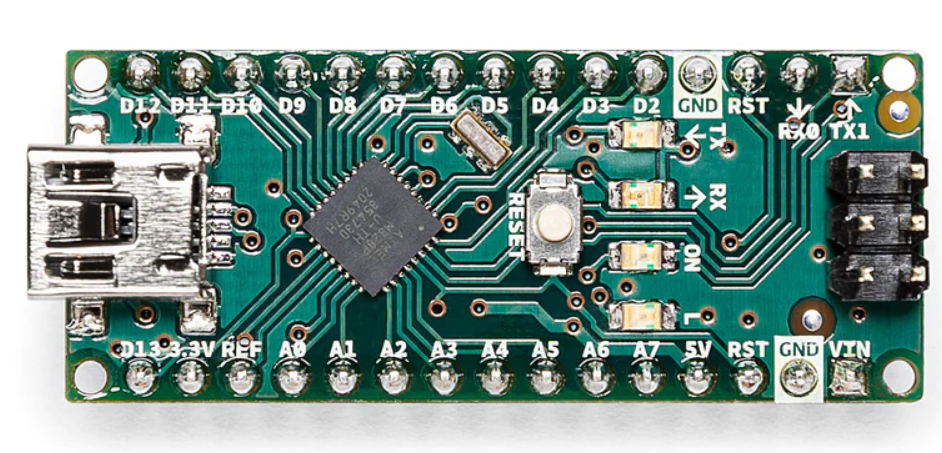
\includegraphics[width=0.4\linewidth]{Pictures/ArduinoNano.png} 
  \caption{Placa de desarrollo Arduino Nano}
  \label{fig:arduinoNanoBoard}
\end{figure}

\begin{table}[b]
\centering
\caption{Especificaciones del Microcontrolador AVR}
\label{tab:nanotable}
\begin{tabular}{l l}
\toprule % Línea horizontal superior
Característica & Valor \\
\midrule % Línea horizontal media
Arquitectura & AVR \\
Voltaje de operación & 5 V \\
Memoria Flash & 32 KB de los cuales 2 KB son utilizados por el bootloader \\
SRAM & 2 KB \\
Velocidad de reloj & 16 MHz \\
Pines de entrada analógica & 8 \\
EEPROM & 1 KB \\
Corriente por pines I/O  & 40 mA (Pines de E/S) \\
Voltaje de alimentación externa & 7-12V \\
Pines digitales I/O & 22 (6 de los cuales son PWM) \\
Salidas PWM  & 6 \\
Consumo de potencia & 19 mA \\
\bottomrule % Línea horizontal inferior
\end{tabular}
\end{table}

\newpage

\section{Datalogger}
Para el registro de datos, hemos optado por el módulo SparkFun OpenLog de código abierto. Este datalogger se comunica a través de una sencilla conexión serie y es compatible con tarjetas microSD de hasta 32 GB. Desempeña la función de un registro de datos, similar a una 'caja negra', capaz de almacenar información generada por nuestro sistema (ver Fig. \ref{fig:datalogger}). En el contexto del EPS, este módulo será responsable de almacenar datos eléctricos, como voltaje y corriente, así como datos ambientales, incluyendo temperatura y presión.

El módulo SparkFun OpenLog está equipado con un ATmega328 que opera a 16 MHz gracias a un oscilador incorporado. En modo inactivo, consume aproximadamente 2-3 mA cuando no hay datos que registrar. Durante una sesión de registro completa, el consumo de energía varía entre 10 y 20 mA, dependiendo del tipo de tarjeta microSD utilizada. Es compatible con tarjetas microSD que tienen una capacidad de 512 MB a 32 GB (ver Tabla \ref{tab:openlog_sparkfun_tabla_specs})\cite{sparkfun-13712}.



\begin{table}[h]
\centering
\caption{Especificaciones del SparkFun OpenLog}
\label{tab:openlog_sparkfun_tabla_specs}
\begin{tabular}{l l}
\toprule
Voltaje de operación & 3V a 5V \\
Velocidad del Microcontrolador & 16 MHz \\
Consumo en Modo Inactivo & 2-3 mA \\
Consumo durante Registro & 10-20 mA \\
Compatibilidad de Tarjetas microSD & 512 MB a 32 GB \\
Formatos de Tarjetas SD & FAT16 y FAT32 \\
\bottomrule
\end{tabular}
\end{table}


\begin{figure}[htbp]
  \centering
  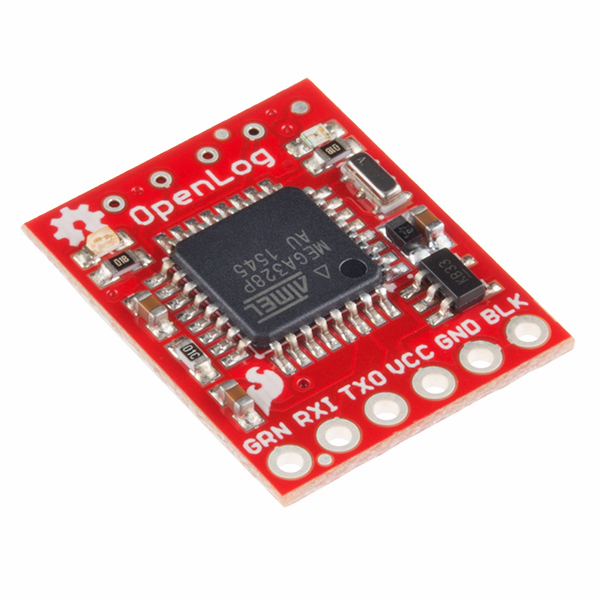
\includegraphics[width=0.4\linewidth]{Pictures/datalogger.jpg} 
  \caption{Módulo Datalogger Openlog de Sparkfun}
  \label{fig:datalogger}
\end{figure}


% Codigo de Prueba de Arduino IDE
\newpage
\begin{lstlisting}[caption={Prueba unitaria de Sparkfun Openlog desarrollado en Arduino IDE}, label={lst:ejemplo}]
#include <SoftwareSerial.h>

SoftwareSerial OpenLog(6, 5);

int statLED = 13;
float dummyVoltage = 3.50;

void setup() {
  pinMode(statLED, OUTPUT);
  Serial.begin(9600);
  OpenLog.begin(9600);

  Serial.println("This serial prints to the COM port");
  OpenLog.println("This serial records to the OpenLog text file");

  OpenLog.println("Hi there! How are you today?");
  OpenLog.print("Voltage: ");
  OpenLog.println(dummyVoltage);
  dummyVoltage++;
  OpenLog.print("Voltage: ");
  OpenLog.println(dummyVoltage);

  Serial.println("Text written to file. Go look!");
}
void loop() {
  digitalWrite(statLED, HIGH);
  delay(1000);
  digitalWrite(statLED, LOW);
  delay(1000);
}

}
\end{lstlisting}

% Codigo de Prueba de Arduino IDE 

\section{Etapa de Potencia}

Esta etapa incorpora un circuito de electrónica de potencia para gestionar la conexión y desconexión de cargas mediante señales digitales del microcontrolador. Se han establecido dos etapas de potencia: una para el bus de 3.3V, alimentando cargas descritas en la Tabla \ref{tab:cuadro_cargas_payload33}, y otra para el bus de 5.0V, para cargas detalladas en la Tabla \ref{tab:cuadro_cargas_payload50}

\begin{table}[h]
    \centering
    \renewcommand{\arraystretch}{1}
    \caption{Carga útil conectada a bus de 3.3v}
    \label{tab:cuadro_cargas_payload33}
    \begin{tabularx}{\textwidth}{lllllll}
    \hline
    \textbf{Descripción} & \textbf{Cantidad} & \textbf{I [mA]} & \textbf{P [W]} & \textbf{t [h]} & \textbf{E [Wh]} & \textbf{Q [mAh]} \\
    \hline
    \text{MCU 3} & 1 unidad & 70.00 & 0.23 & 2.00 & 0.46 & 140.00 \\ 
    \text{Cámara IR} & 1 unidad & 25.00 & 0.08 & 2.00 & 0.17 & 50.00 \\\hline 
    & \textbf{I Máx.} & \text{95.00} & & & & \textbf{190.00} \\ \hline
    \end{tabularx}
\end{table}

\begin{table}[h]
    \centering
    \renewcommand{\arraystretch}{1}
    \caption{Carga útil conectada a bus de 5.0v}
    \label{tab:cuadro_cargas_payload50}
    \begin{tabularx}{\textwidth}{lllllll}
        \hline
        \textbf{Descripción} & \textbf{Cantidad} & \textbf{I [mA]} & \textbf{P [W]} & \textbf{t [h]} & \textbf{E [Wh]} & \textbf{Q [mAh]} \\
        \hline
        Cámara & 1 unidad & 260.00 & 1.30 & 2.00 & 2.60 & 520 \\
        Datalogger 2 & 1 unidad & 12.00 & 0.06 & 2.00 & 0.12 & 24\\\hline
        ~ & \textbf{I Máx.} & \text{282.00} & ~ & ~ & ~ & \textbf{544.00} \\
        \hline
    \end{tabularx}
\end{table}

En el ámbito de la electrónica, las opciones de diseño abarcan soluciones que incorporan bobinas, como los relés y dispositivos semiconductores, como los transistores \cite{rashid2015electronica}. En el contexto de este trabajo de investigación, la elección de utilizar relés fue descartada debido a la significativa disipación de potencia por efecto Joule asociada con la operación de las bobinas. Esta decisión se respalda con ejemplos específicos de soluciones comerciales, como el relé PE014006, capaz de disipar hasta 209 mW \cite{TE2023PE014006}, un nivel de disipación que resulta inaceptable en aplicaciones alimentadas por baterías.


En consecuencia, dirigimos nuestra atención hacia alternativas basadas en semiconductores, específicamente los transistores. Entre estos, los BJT y los MOSFET son considerados mayoritariamente debido a su disponibilidad y asequibilidad. Mientras que el BJT es controlado por corriente, el MOSFET responde al control por voltaje. Las diferencias fundamentales entre estos dispositivos se resumen de manera concisa en la Tabla \ref{tab:comparisonbjtmosfet}.

Con el objetivo de realizar un análisis más directo y preciso, optamos por dos modelos comerciales accesibles: el BJT 2N2222A (Fig. \ref{fig:subfig12N2222A}) y el MOSFET BS170 (Fig. \ref{fig:subfig2bs170}).
\newpage

\begin{table}[h]
    \centering
    \renewcommand{\arraystretch}{1.5}
    \begin{tabular}{p{0.35\linewidth}p{0.25\linewidth}p{0.30\linewidth}}
    \hline
        \textbf{Característica} & \textbf{BJT} & \textbf{MOSFET} \\ \hline
        Tipo & PNP/NPN & N/P \\ 
        Control & Corriente & Voltaje \\ 
        Temp. Coeficiente & Negativo & Positivo \\ 
        Salida controlada & Corriente de base & Voltaje en compuerta\\ 
        Costo & Bajo & Alto \\ 
        Descarga electrostática & No problema & Problema potencial \\ 
        Ganancia de corriente & Baja e inestable & Alta y estable \\ 
        Resistencia de entrada & Baja & Alta \\ 
        Corriente de entrada & mA/uA & pA \\ 
        Velocidad de conmutación & Más lenta & Más rápida \\ 
        Impedancia de entrada & Baja & Alta \\ 
        Frecuencia de conmutación & Baja & Alta \\ 
        Aplicaciones & Baja corriente & Alta corriente \\ \hline
    \end{tabular}
    \caption{Características generales de BJT y MOSFET.}
    \label{tab:comparisonbjtmosfet}
\end{table}

\vspace{1 cm}

\begin{figure}[h]
  \centering
  \begin{subfigure}{0.4\textwidth}
    \centering
    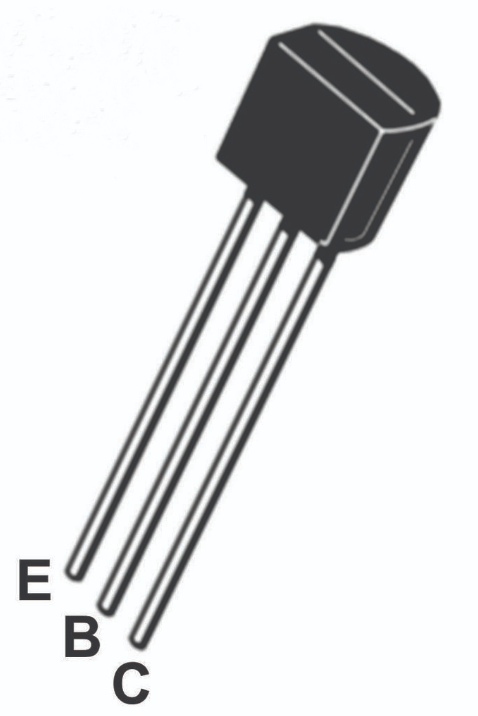
\includegraphics[width=0.7\linewidth]{Pictures/2N2222A_Pinout.png}
    \caption{BJT 2N2222A}
    \label{fig:subfig12N2222A}
  \end{subfigure}
  \hspace{2cm} % Ajusta el espacio entre las subfiguras
  \begin{subfigure}{0.4\textwidth}
    \centering
    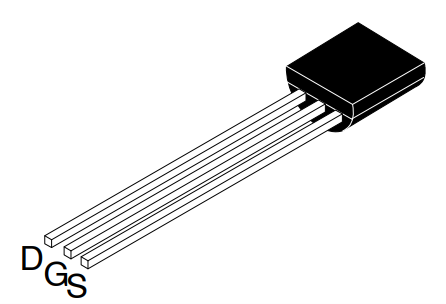
\includegraphics[width=0.9\linewidth]{Pictures/BS170_Pinout.png}
    \caption{MOSFET BS170}
    \label{fig:subfig2bs170}
  \end{subfigure}
  \caption{Transistores BJT y MOSFET comerciales}
  \label{fig:arduinoNanoSubfigures}
\end{figure}

\newpage

\subsection{Análisis Comparativo entre BJT 2N2222A y MOSFET BS170}

Con el objetivo de realizar una comparación precisa entre los transistores BJT 2N2222A y MOSFET BS170, es imperativo establecer criterios relevantes que orienten la evaluación:

\begin{itemize}
\item Capacidad de corriente en drenaje o colector.
\item Rango de temperatura de operación.
\item Potencia disipada.
\item Resistencia térmica.
\end{itemize}

Para facilitar la elaboración de una tabla comparativa directa entre ambos modelos, nos apoyaremos en las hojas técnicas respectivas proporcionadas en \cite{BS170Datasheet} y \cite{2N2222A_Datasheet}.

\begin{table}[h]
    \centering
    \begin{tabularx}{\textwidth}{lcc}
        \hline
        \textbf{Parámetro} & \textbf{BS170} & \textbf{2N2222A} \\ 
        \hline
        Corriente Máxima ($I_{\text{Máx.}}$) & \SI{500}{\milli\ampere} & \SI{600}{\milli\ampere} \\ 
        Potencia Disipada ($P_D$) & \SI{830}{\milli\watt} a \SI{6.60}{\milli\watt/\celsius} & \SI{625}{\milli\watt} a \SI{5.0}{\milli\watt/\celsius} \\ 
        Potencia Disipada ($P_D$) & \SI{830}{\milli\watt} a \SI{6.60}{\milli\watt/\celsius}  & \SI{1.5}{\watt} a \SI{12.0}{\milli\watt/\celsius} \\ 
        Rango de Temperatura & \SI{-55}{\celsius} a \SI{+150}{\celsius} & \SI{-55}{\celsius} a \SI{+150}{\celsius} \\ 
        R$\theta$ja & \SI{150}{\celsius/\milli\watt} & \SI{200}{\celsius/\milli\watt} \\ 
        \hline
    \end{tabularx}
    \caption{Comparativa entre MOSFET BS170 y BJT 2N2222A.}
    \label{tab:comparisonmodeltransistor}
\end{table}

En la Tabla \ref{tab:comparisonmodeltransistor} se detallan las características clave de los modelos de transistores seleccionados. El BJT 2N2222A, al ser un dispositivo de coeficiente térmico negativo (NTC), muestra incremento en la resistencia interna con la disminución de la temperatura ambiente (Fig. \ref{fig:pdenviromentaltemperature}). En contraste, los transistores MOSFET, como el BS170, son PTC y disminuyen su resistencia a bajas temperaturas (Fig. \ref{fig:resinternavscorriente}).

Ambos transistores admiten un amplio rango de temperaturas, pero el BJT permite una corriente más alta y tiene un incremento térmico significativamente mayor. Sin embargo, considerando el consumo de energía crítico para baterías, la respuesta más eficiente del MOSFET a la temperatura lo posiciona como la mejor alternativa.

En conclusión, para la aplicación específica en la misión de globo de gran altitud de StratoBalloon, se favorece la implementación del MOSFET BS170 en la etapa de potencia, debido a su eficiencia energética y respuesta térmica más favorable.

\newpage

\begin{figure}[h]
  \centering
  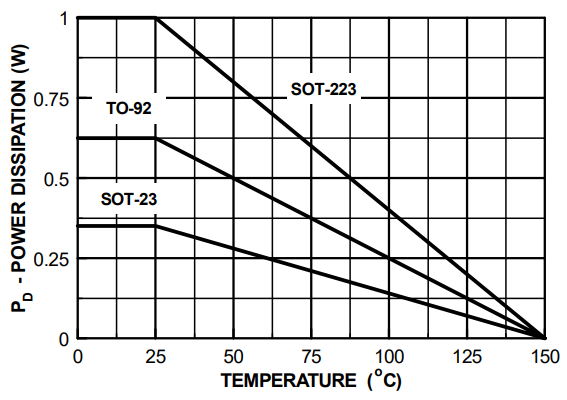
\includegraphics[width=0.85\linewidth]{Pictures/2N2222ApowerD.png} 
  \caption{Variación de la Potencia Disipada en el 2N2222A en Función de la Temperatura Ambiente \cite{2N2222A_Datasheet}}
  \label{fig:pdenviromentaltemperature}
\end{figure}

\begin{figure}[h]
  \centering
  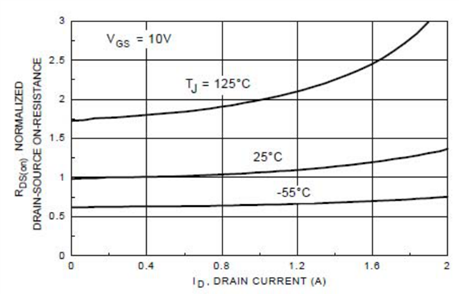
\includegraphics[width=0.9\linewidth]{Pictures/resvscorriente.png} 
  \caption{Variación de la Resistencia Interna en Función de la Corriente a Distintas Temperaturas Ambiente para un MOSFET BS170 \cite{BS170Datasheet}}
  \label{fig:resinternavscorriente}
\end{figure}

\newpage

\subsection{Diseño e implementación de MOSFET BS170}
    

Considerando las indicaciones del fabricante \cite{BS170Datasheet}, se han identificado parámetros fundamentales para el diseño de la etapa de potencia con el MOSFET BS170. Destaca el voltaje máximo $V_{DS}$ entre Drenaje y Fuente, limitado a 60 V, así como el máximo voltaje $V_{GS}$ soportado en la compuerta, establecido en 20 V.

Un aspecto clave es $V_{GS}(TH)$, definiendo el rango típico de voltajes para activar la compuerta y permitir la conducción, sujeto a una curva de comportamiento en relación con la corriente en el Drenaje2. Además, se aborda $I_{D}(Load) Máx$, indicando la corriente máxima en el Drenaje, asociada con la carga máxima manejable.

Estos aspectos esenciales se detallan en la Tabla \ref{tab:Designbs170}, proporcionando información crucial para un diseño eficiente y seguro de la etapa de potencia.

\begin{table}[!ht]
    \centering
    \begin{tabular}{l l}
    \hline
        \textbf{Parámetro} & \textbf{Valor} \\ \hline
        V\_DS (BR) & 60 V \\ 
        V\_GS  MAX & 20 V \\ 
        V\_GS Threshold & Min. 0.8 – 2.1 avg – 3 Máx \\ 
        I\_D (Load) MAX & 500 mA \\ 

        I\_DSS & 10 nA \\ 
        I\_DM & 1200 mA \\ 
    \hline
    \end{tabular}
    \caption{Parámetros de diseño para MOSFET BS170}
    \label{tab:Designbs170}
\end{table}

De acuerdo a la documentación técnica del MOSFET BS170 \cite{BS170Datasheet}, y basándonos en la Figura \ref{fig:bs170vgsidrainA}, seleccionamos el valor mínimo de $V_{GS}$ necesario para el BS170 en el bus de 3.3 V, considerando una corriente aproximada de 100 mA. Asimismo, elegimos el voltaje mínimo $V_{GS}$ para la etapa de potencia en el bus de 5.0 V, con una corriente mínima de 300 mA. En ambos casos, y al verificar que los valores son aceptables según se muestra en la Tabla \ref{tab:Designbs170}, optamos por utilizar el voltaje suministrado naturalmente por el Arduino Nano, que es de 5 VDC con una corriente máxima continua de 20 mA \cite{arduino_getting_started}.

Dicho esto, siguiendo la conexión del MOSFET en la configuración "low side" para este MOSFET de canal N, permitiendo así que funcione como un interruptor normalmente abierto y se active en función de una señal de entrada del microcontrolador, el esquemático y vista 3D de la PCB resultante se muestran en la Figura \ref{fig:combined_figureBS170}.

\newpage

\begin{figure}[h]
  \centering
  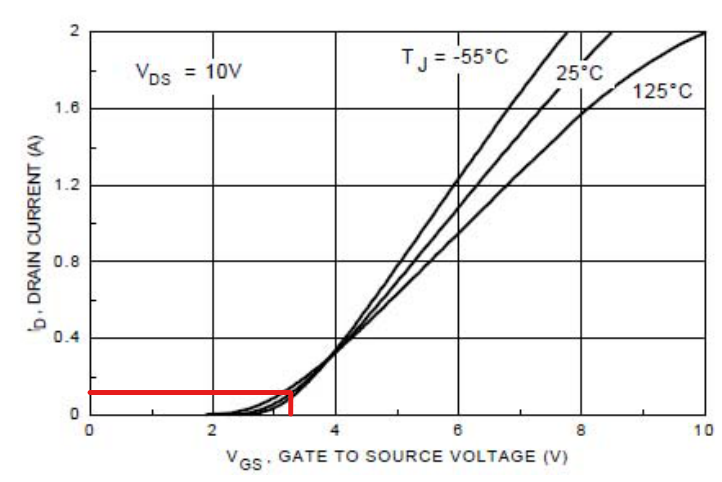
\includegraphics[width=0.45\linewidth]{Pictures/33busvgsgraphic.png} 
  \caption{$V_{GS}$ para bus de 3.3 V a 100 [mA]. \cite{BS170Datasheet}}
  \label{fig:bs170vgsidrainA}
\end{figure}

\begin{figure}[h]
  \centering
  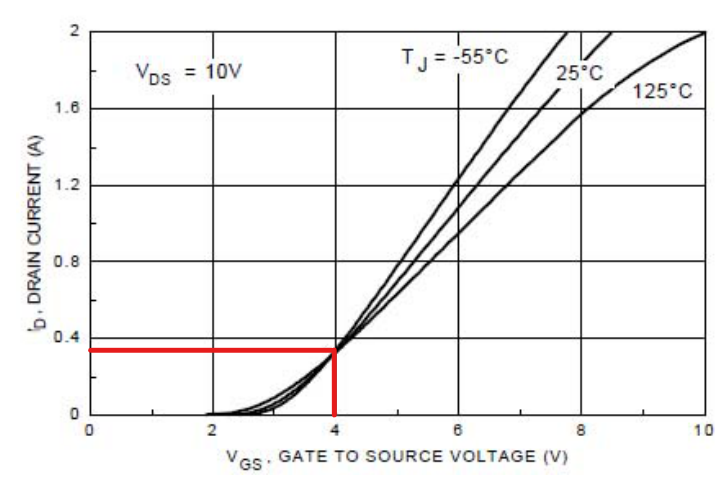
\includegraphics[width=0.45\linewidth]{Pictures/50busvgsgraphic.png} 
  \caption{$V_{GS}$ para bus de 5.0 V a 300 [mA]. \cite{BS170Datasheet}}
  \label{fig:bs170vgsidrainB}
\end{figure}

\vspace{1 cm }

\begin{figure}[h]
    \centering
    \begin{subfigure}{0.45\textwidth}
        \centering
        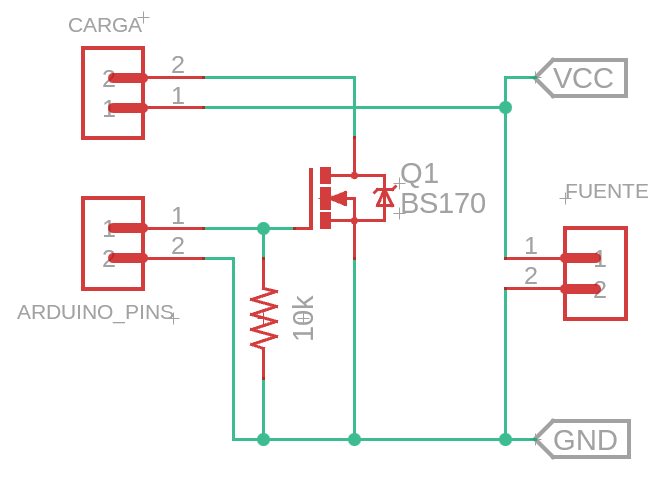
\includegraphics[width=\linewidth]{Pictures/EtapaMosfet_Esquematico.png}
        \caption{Esquemático de la etapa de potencia con MOSFET BS170. La resistencia de 10k ohmios es un valor recomendado por el fabricante \cite{BS170Datasheet}.}
        \label{fig:Esquematico_powerstage170}
    \end{subfigure}
    \hfill
    \begin{subfigure}{0.45\textwidth}
        \centering
        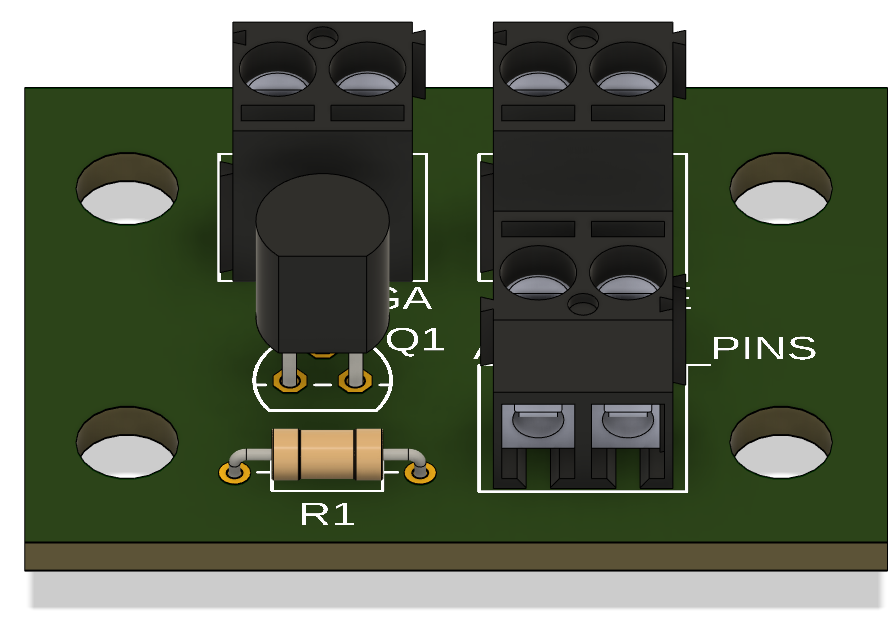
\includegraphics[width=\linewidth]{Pictures/3D_MOSFET.png}
        \caption{Vista 3D de la etapa de potencia con MOSFET BS170.}
        \label{fig:3Do_powerstage170}
    \end{subfigure}
    \caption{Esquemático y vista 3D de la etapa de potencia con MOSFET BS170.}
    \label{fig:combined_figureBS170}
\end{figure}


\newpage


\section{Instrumentación}

\subsection{Barómetro y sensor de temperatura}

Para llevar a cabo la medición de presión y temperatura durante la misión, así como para realizar un análisis comparativo con respecto al rendimiento frente a parámetros eléctricos, hemos optado por la utilización del sensor de bajo costo MS5611. Las especificaciones detalladas de este sensor se presentan en la Tabla \ref{tab:ms5611}.

El código de programación utilizado para realizar la prueba unitaria de este componente se encuentra detallado en el Código 4.2.


\begin{table}[h]
\centering
\caption{Especificaciones sensor MS5611}
\label{tab:ms5611}
\begin{tabular}{ll}
\toprule
Rango de presiones & 10 to 1200 mbar \\
Rango de temperaturas & -40 °C to 85 °C \\
Resolución en altura & 10 cm \\
Resolución en presión & 0.012 mbar \\
Resolución en temperatura & 0.01 °C \\
Fuente de alimentación & 1.8 to 3.6 V \\
Consumo en corriente & 1.4 mA \\
Comunicación & I²C y SPI \\
\bottomrule
\end{tabular}
\end{table}

% Codigo de Prueba de Arduino IDE

\begin{lstlisting}[caption={Prueba unitario en sensor MS5611 desarrollado en Arduino IDE}, label={code:ms5611cod}]
#include <Wire.h>
#include <MS5611.h>

MS5611 ms5611;
double referencePressure;

void setup() 
{
  Serial.begin(9600);
  Serial.println("Initialize MS5611 Sensor");
  
  while (!ms5611.begin())
  {
    Serial.println("Could not find a valid MS5611 sensor, check wiring!");
    delay(500);
  }
  
  referencePressure = ms5611.readPressure();
  checkSettings();
}

void checkSettings()
{
  Serial.print("Oversampling: ");
  Serial.println(ms5611.getOversampling());
}

void loop()
{
  uint32_t rawTemp = ms5611.readRawTemperature();
  uint32_t rawPressure = ms5611.readRawPressure();
  
  double realTemperature = ms5611.readTemperature();
  long realPressure = ms5611.readPressure();
  
  float absoluteAltitude = ms5611.getAltitude(realPressure);
  float relativeAltitude = ms5611.getAltitude(realPressure, referencePressure);
  
  String logData = String(realTemperature, 2) + " *C, " + String(realPressure) + " Pa; ";
  logData += "Absolute Altitude: " + String(absoluteAltitude, 2) + " m; ";
  
  Serial.println(logData);
  delay(1000);

}
\end{lstlisting}

% Codigo de Prueba de Arduino IDE 


\subsection{Medidor de voltaje}

Para medir los voltajes del banco de baterías del Sistema de energía (EPS), hemos elegido utilizar el Convertidor Analógico-Digital (ADC) integrado en el Arduino Nano. El ADC del Arduino Nano ofrece una resolución de 10 bits, lo que permite mediciones precisas con una sensibilidad de 4.88 mV por unidad de conteo (4.88 mV/count). A continuación, presentamos un código de prueba unitaria para la medición de voltajes (ver Código 4.3). Los parámetros técnicos asociados al ADC se detallan en Tabla \ref{tab:ArduinoADC}.

\begin{table}[h]
\centering
\caption{Especificaciones del ADC del Arduino Nano}
\label{tab:ArduinoADC}
\begin{tabular}{llll}
\toprule
\textbf{Placa} & \textbf{Voltaje de Operación} & \textbf{Pines} & \textbf{Resolución Máx.} \\
\midrule
Nano & 5 Voltios & A0 a A5 & 10 bits \\
\bottomrule
\end{tabular}
\end{table}


% Codigo de Prueba de Arduino IDE

\begin{lstlisting}[caption={Prueba unitaria para ADC desarrollado en Arduino IDE}, label={lst:ADCode}]
const int pinAnalogico = A0;

void setup() {
  Serial.begin(9600);
}

void loop() {
  int lectura = analogRead(pinAnalogico);
  float voltaje = (lectura * 5.0) / 1023.0;

  Serial.print("Valor: ");
  Serial.print(lectura);
  Serial.print(", Voltaje: ");
  Serial.println(voltaje, 2);

  delay(1000);
}

\end{lstlisting}

% Codigo de Prueba de Arduino IDE 

\newpage
\subsection{Medidor de corriente}

Para la medición precisa de corriente sin afectar el circuito, hemos optado por el uso del sensor ACS723 (ver Fig.\ref{fig:Sensor_ACS723_Imagen} ), una placa de alta precisión diseñada para aplicaciones de corriente AC y DC, que utiliza el efecto Hall para generar una tensión proporcional a la corriente que fluye a través de sus pines IP+ e IP-. Una ventaja fundamental es que el sensor emplea un efecto Hall, lo que proporciona un aislamiento eléctrico entre el circuito medido y el circuito que lee el sensor. Esto significa que, aunque nuestro Arduino funcione a 5V, el circuito medido puede operar a tensiones DC o AC más elevadas.

\begin{figure}[h]
  \centering
  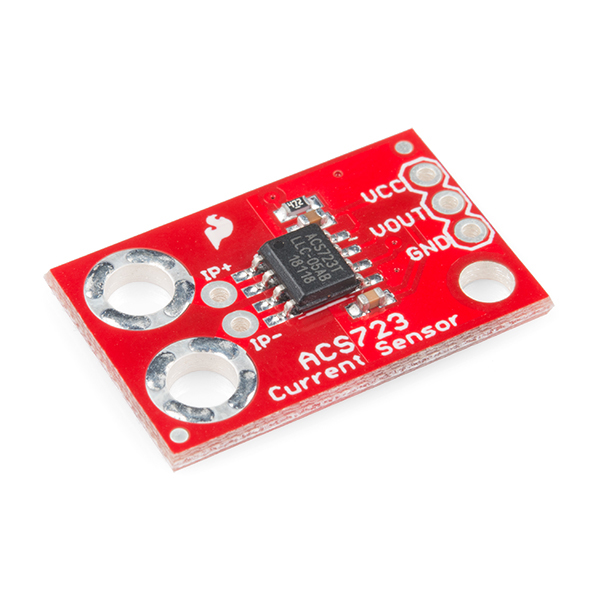
\includegraphics[width=0.7\linewidth]{Pictures/ACS723.jpg} 
  \caption{Sensor ACS723 de Sparkfun.}
  \label{fig:Sensor_ACS723_Imagen}
\end{figure}


Este sensor de baja corriente puede detectar corrientes muy pequeñas, incluso a partir de 10mA, y corrientes más altas de hasta 5A. No obstante, dado que su salida es analógica, la precisión de las lecturas estará limitada por el ruido y la resolución del convertidor analógico-digital (ADC) que lee la señal. Además, esta placa ofrece aislamiento eléctrico completo entre los circuitos medidos y de detección y, gracias a un amplificador integrado, permite ajustar su sensibilidad \cite{sparkfun14544}.

A continuación, presentamos un código de prueba unitaria para la medición de corrientes utilizando este dispositivo (ver Código 4.4).


% Codigo de Prueba de Arduino IDE

\begin{lstlisting}[caption={Prueba unitaria para sensor de corriente ACS723}, label={lst:acs723cod}]

const int analogInPin = A0;
const int avgSamples = 10;
int sensorValue = 0;
float sensitivity = 100.0 / 500.0; 
float Vref = 2500;

void setup() {
  Serial.begin(9600);
}

void loop() {
  for (int i = 0; i < avgSamples; i++) {
    sensorValue += analogRead(analogInPin);
    delay(2);
  }
  sensorValue = sensorValue / avgSamples;

  float voltage = 4.88 * sensorValue;
  float current = (voltage - Vref) * sensitivity;

  Serial.print(current);
  Serial.print("mA");
  Serial.print(analogRead(A1));
  Serial.print("mV_Resistor");

  Serial.print("\n");
  
  sensorValue = 0;
}


\end{lstlisting}

% Codigo de Prueba de Arduino IDE 

\newpage



\section{Baterías}

La selección de baterías de iones de litio comerciales (COTS, por sus siglas en inglés) adecuadas para misiones en globos de gran altitud es una consideración crítica. Si bien las baterías COTS ofrecen rentabilidad, amplia disponibilidad y un historial probado en diversas aplicaciones, se deben abordar cuidadosamente los desafíos únicos de operar a altitudes extremas. Las misiones en globos de gran altitud requieren un rendimiento confiable de las baterías, incluso bajo condiciones ambientales adversas e impredecibles.

Las bajas temperaturas y presiones pueden afectar significativamente el rendimiento de las baterías, comprometiendo potencialmente la seguridad de la misión. Operar baterías en tales condiciones conlleva efectos perjudiciales, incluyendo la alteración de la conductividad iónica, la resistencia interna y la cinética de transferencia de carga\cite{Ma2018,Navarathinam2011}. Dada la importancia de la energía de la batería para los sistemas electrónicos durante las misiones en globos de gran altitud, evaluar las baterías de iones de litio COTS es esencial para garantizar el éxito de la misión.

\subsection{Química y geometría de las baterías}\label{AA} 

A pesar de su tamaño compacto, alta densidad de energía y baja tasa de autodescarga, las baterías de iones de litio conllevan riesgos potenciales inherentes, como posibles incendios o explosiones debido a cortocircuitos internos \cite{Meyer2020}.

En cuanto a la geometría de la batería, los diseños prismáticos optimizan la utilización del espacio, pero a menudo requieren mejoras en la eficiencia térmica. Las baterías de tipo bolsa ofrecen flexibilidad en su forma, aunque necesitan un soporte adecuado. Por otro lado, las baterías cilíndricas, como las del tipo 18650, proporcionan estabilidad mecánica y cuentan con sistemas de seguridad integrados, lo que las hace especialmente adecuadas para aplicaciones en globos de gran altitud\cite{Eleazar2020}.

\subsection{Baterías comerciales}

\vspace{0.5cm}
\begin{figure}[htbp]
  \centering
  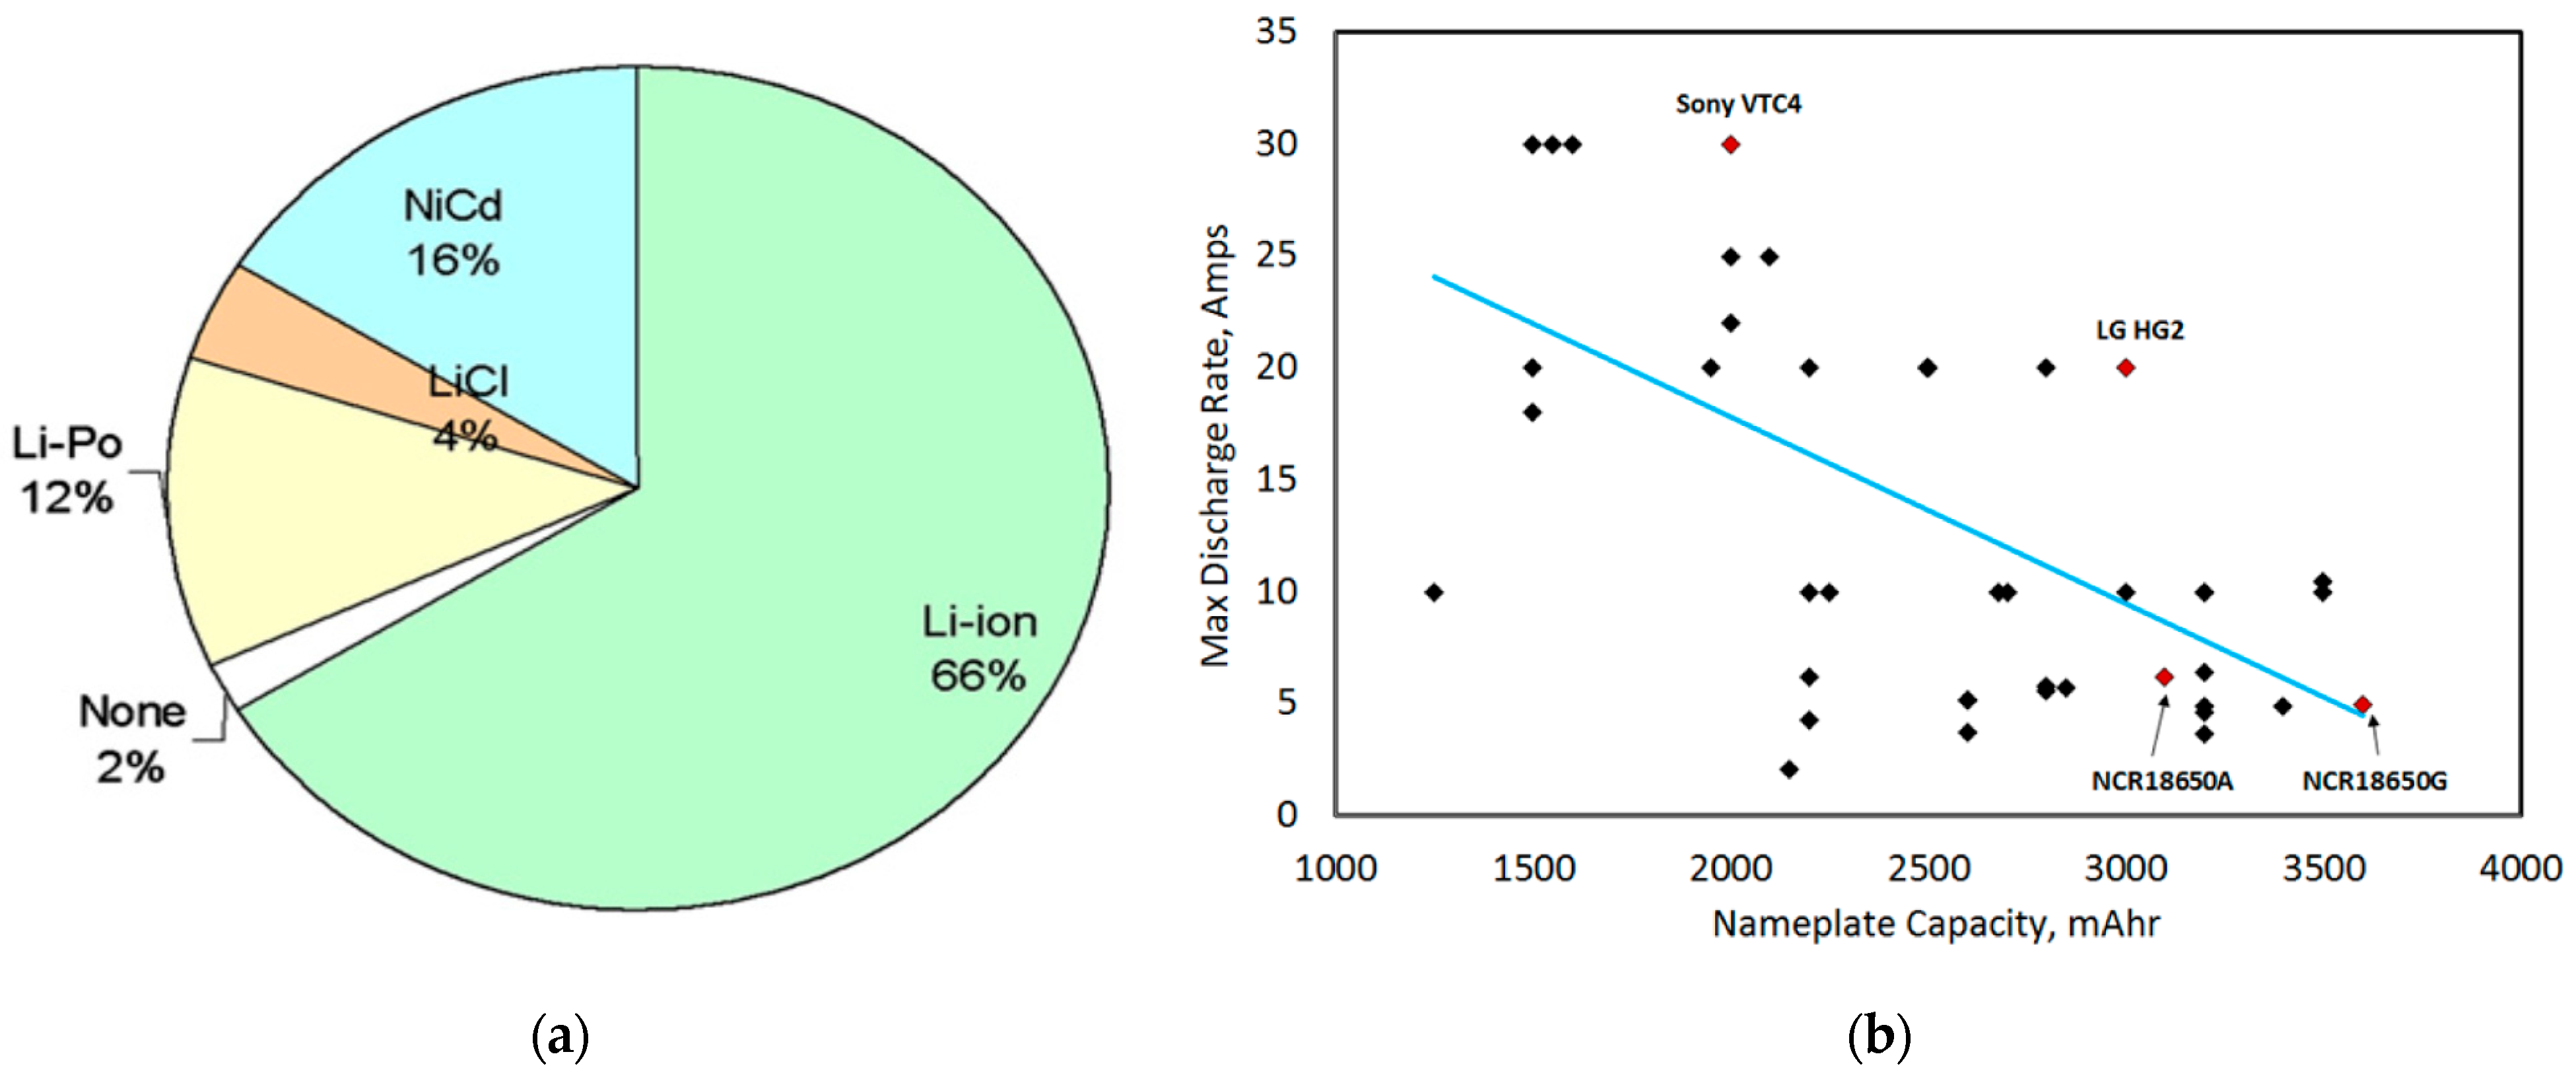
\includegraphics[width=0.9\linewidth]{Pictures/COTSBatteries.png} 
  \caption{(a) Battery types used in pico- and nano-satellites\cite{bouwmeester2010survey}.
  (b) Summary of maximum discharge rate capabilities versus nameplate capacity of some representative COTS 18650 Li-ion cells \cite{chin2018energy}}
  \label{fig:graphicsCOTS}
\end{figure}

Basándonos en el estudio exhaustivo realizado en \cite{Knap2020} y representado en la Fig. \ref{fig:graphicsCOTS}, el rendimiento de las celdas de iones de litio puede ser efectivamente limitado por tres modelos específicos: Sony VTC4, LG HG2 y Panasonic NCR18650G.

Debido a su costo asequible, historial comprobado de confiabilidad y características electroquímicas de carga y descarga, hemos optado por utilizar la batería Panasonic NCR18650B en este trabajo. \newpage Esta batería tiene una capacidad de descarga de hasta 4.9A, una capacidad de carga de 3400 mAh y un rango de temperatura de -20 a 60 grados Celsius\cite{panasonic_18650b}. Además, cuenta con documentación técnica que respalda su uso en aplicaciones aeroespaciales previas\cite{Knap2020}\cite{Kumar2022}.

\subsection{Arreglo para el banco de baterías}

Al analizar la Tabla \ref{tab:requerimientos-eps}, que presenta los requerimientos del Sistema de Energía (EPS), obtenidos a partir del presupuesto energético desarrollado en las Tablas \ref{tab:cuadro-cargas1} y \ref{tab:cuadro-cargas2}, se observa que la corriente requerida por las cargas se estima en 1385.4 mA. Tras consultar la hoja técnica del modelo de batería Panasonic NCR18650B utilizado en este trabajo, se verifica que este modelo de batería puede suministrar una corriente máxima de 4.9 A. Por lo tanto, este diseño no está restringido ni obligado a utilizar arreglos en paralelo.

En lo que respecta a las necesidades de capacidad de carga, se ha estimado un valor nominal de 6844.2 mAh para la misión StratoBalloon, sin considerar las posibles pérdidas en las diversas etapas del EPS.

Dado que la capacidad nominal de esta batería es de 3400 mAh, se calcula que se requerirían 3 baterías, considerando un redondeo hacia arriba. No obstante, dado que aún disponemos de espacio y pensando en futuras aplicaciones, hemos decidido utilizar 4 baterías de este tipo.

Con el fin de explorar el funcionamiento de etapas posteriores, como los convertidores DC-DC, se han considerado tres diseños: 4s1p (Fig. \ref{fig:powerbank}), 2s2p (Fig. \ref{fig:powerbank2}) y 1s4p (Fig. \ref{fig:powerbank3}).

\begin{figure}[h]
  \centering
  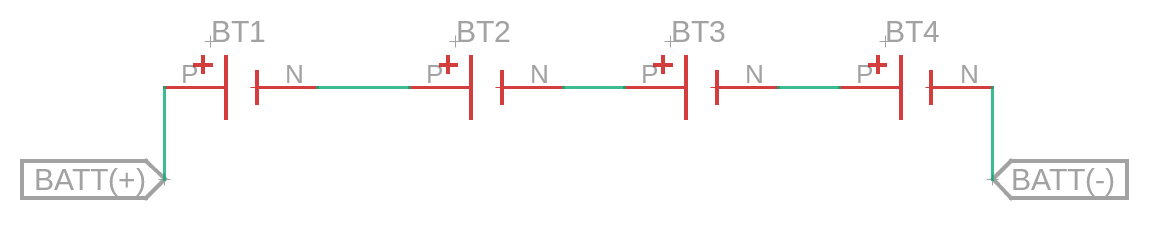
\includegraphics[width=0.7\linewidth]{Pictures/PowerBank.png} 
  \caption{Banco de baterías en arreglo 4s1p a 14.4 V.}
  \label{fig:powerbank}
\end{figure}

\begin{figure}[h]
  \centering
  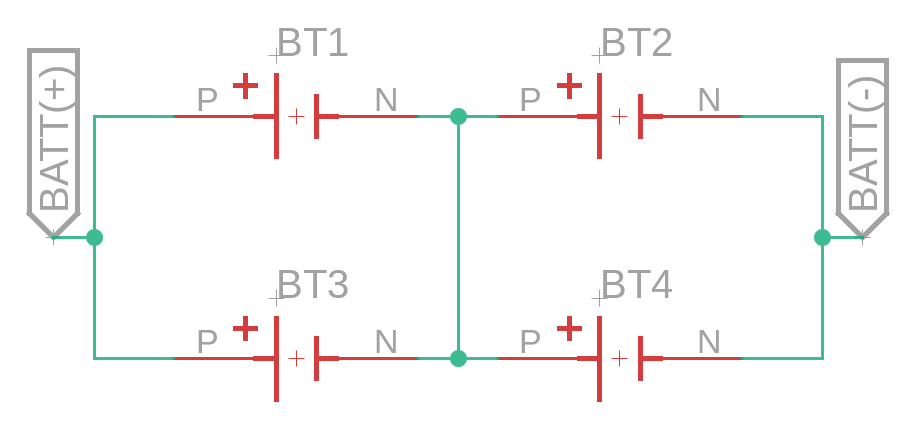
\includegraphics[width=0.5\linewidth]{Pictures/Batteries2s2p.png} 
  \caption{Banco de baterías en arreglo 2s2p a 7.2 V.}
  \label{fig:powerbank2}
\end{figure}

\begin{figure}[h]
  \centering
  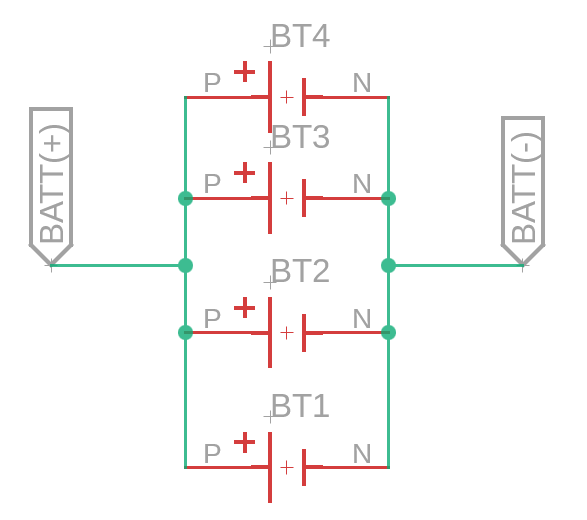
\includegraphics[width=0.4\linewidth]{Pictures/Batteries1s4p.png} 
  \caption{Banco de baterías en arreglo 1s4p a 3.6 V.}
  \label{fig:powerbank3}
\end{figure}

\begin{figure}
  \centering
  \begin{subfigure}{0.35\linewidth}
    \centering
    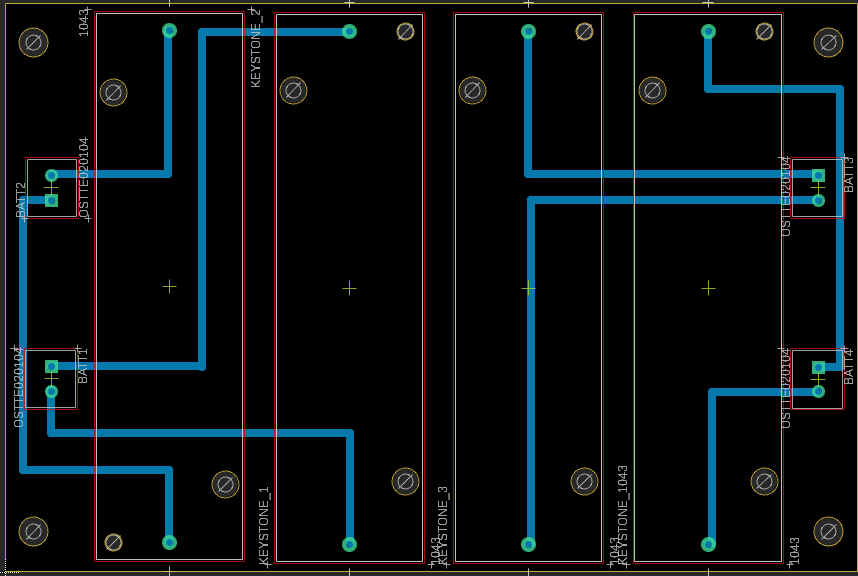
\includegraphics[width=\linewidth]{Pictures/DesignPCBHolders.png}
    \caption{Diseño de pistas}
    \label{fig:powerbankpistas}
  \end{subfigure}
  \begin{subfigure}{0.45\linewidth}
    \centering
    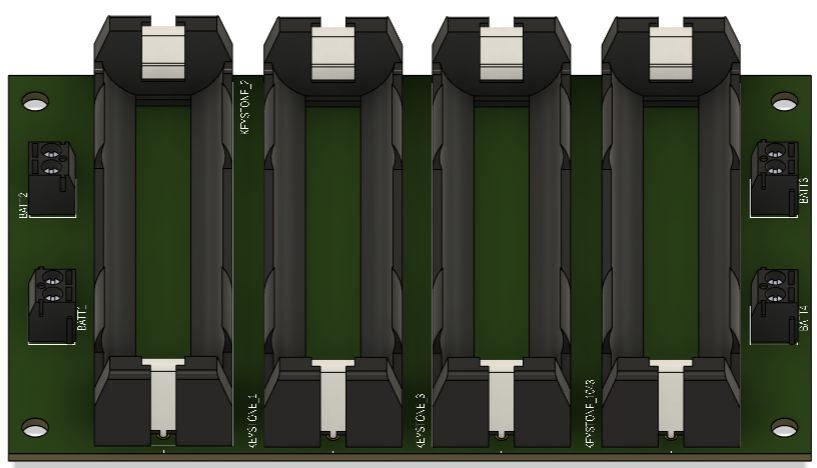
\includegraphics[width=\linewidth]{Pictures/DesignPCBHolders3d.png}
    \caption{Vista 3D de PCB}
    \label{fig:powerbankpistas3d}
  \end{subfigure}
  \caption{Banco de baterías}
  \label{fig:powerbank-subfiguras}
\end{figure}


Para llevar a cabo pruebas preliminares y verificar el rendimiento óptimo en prototipado rápido, hemos instalado en una placa de circuito impreso (PCB) cuatro pilas a través de los portadores Keystone 1043 conectados a bornes para facilitar su manipulación (consulte las Fig. \ref{fig:powerbankpistas} y \ref{fig:powerbankpistas3d}).


\section{Selección del Cargador para el Sistema de Energía (EPS)}

Una vez determinado el tipo de baterías a utilizar en nuestro Sistema de Energía (EPS), la elección de un cargador adecuado se vuelve crucial. Al analizar los resultados de las simulaciones de trayectoria (ver Figura \ref{fig:ruta}), observamos una duración de vuelo relativamente corta, de aproximadamente 2 horas. Debido a esto, se descarta la necesidad de ciclos de carga a bordo, calificando la implementación de un cargador como un requisito deseable pero no indispensable. La selección del cargador dependerá de la evaluación del EPS en conjunto con otros componentes, teniendo en cuenta el propósito del sistema y evitando complicaciones innecesarias.

Al explorar alternativas disponibles, la primera opción considera no desechar la idea de un cargador a bordo. Para esto, consideramos el circuito integrado MCP73831T-2ACI/OT, un controlador de carga lineal diseñado para baterías de iones de litio con un voltaje nominal de 3.6 V \cite{MCP73831-datasheet,sparkfun-10217}.

La corriente de carga se ajusta mediante una resistencia externa siguiendo la ecuación \ref{eq:corriente_carga}

\begin{equation}\label{eq:corriente_carga}
    I_{\text{Reg}} = \frac{1000[V]}{Resistencia_{\text{Externa}[k\Omega]}}
\end{equation}

Dado que la corriente máxima es de 500 mA, se configura con dicho valor mediante una resistencia equivalente de 2 kOhm (consultar ecuación \ref{eq:corriente_configurada}), el esquemático resultante se muestra en la Fig. \ref{fig:cargador}.

\begin{equation}\label{eq:corriente_configurada}
    I_{\text{Reg}} = \frac{1000[V]}{2 \text{[k}\Omega\text{]}} = 500 \text{[mA]}
\end{equation}

\begin{figure}[h]
  \centering
  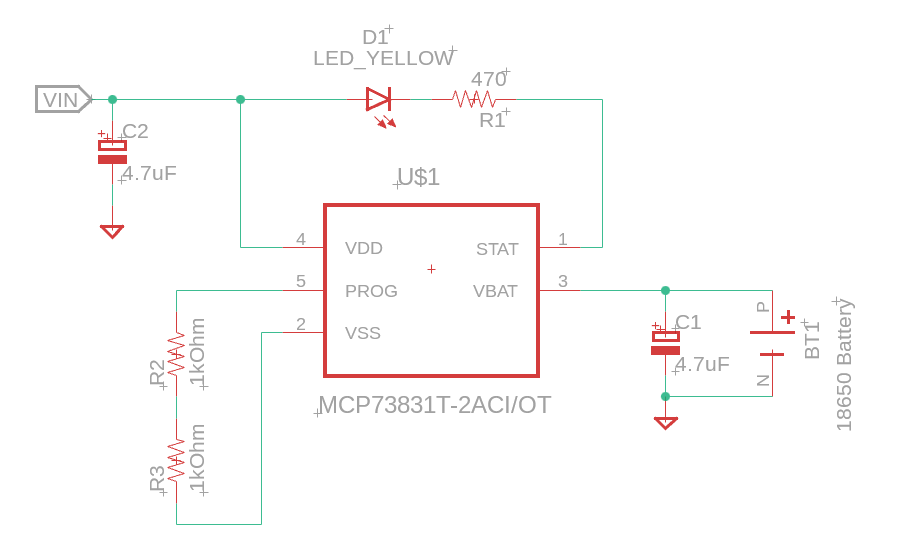
\includegraphics[width=0.75\linewidth]{Pictures/Circuito_cargador.png} 
  \caption{Circuito de carga MCP73831T-2ACI/OT configurado a 500 mA. }
  \label{fig:cargador}
\end{figure}

Es importante destacar que este cargador lineal está diseñado para una sola celda, por lo que se deberá implementar el circuito la misma cantidad de veces acorde a la cantidad de baterías.

Para realizar pruebas preliminares y verificar el rendimiento mediante prototipado rápido, hemos instalado en una placa de circuito impreso (PCB) el circuito cargador, para poder trabajar en conjunto con la PCB del arreglo de baterías (consultar Figuras \ref{fig:Chargerpistas} y \ref{fig:Charger3d}).

\begin{figure}
  \centering
  \begin{subfigure}{\linewidth}
    \centering
    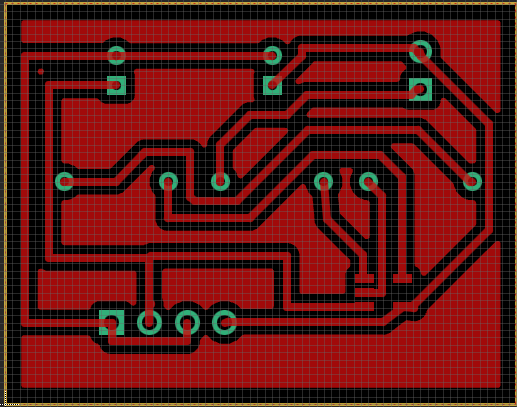
\includegraphics[width=0.4\linewidth]{Pictures/DesignPCBCharger.png}
    \caption{Diseño de pistas cargador MCP73831T-2ACI/OT}
    \label{fig:Chargerpistas}
  \end{subfigure}
  \begin{subfigure}{\linewidth}
    \centering
    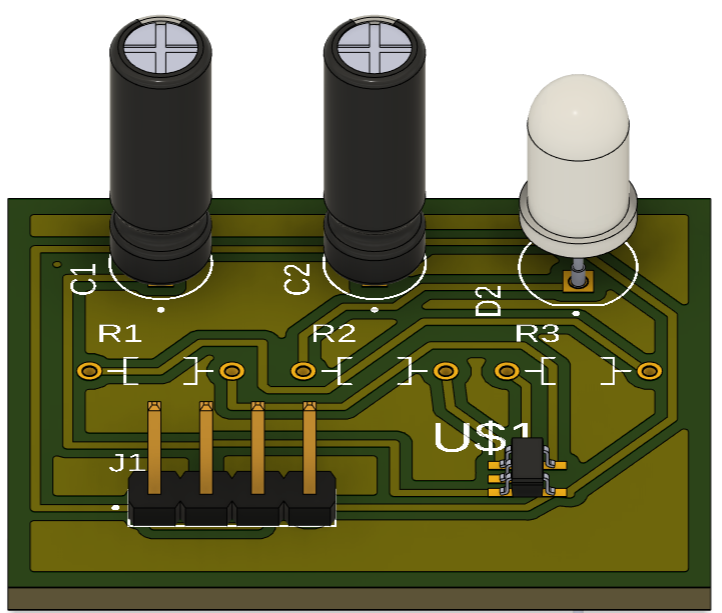
\includegraphics[width=0.4\linewidth]{Pictures/DesignPCBCharger3d.png}
    \caption{Vista 3D de PCB MCP73831T-2ACI/OT}
    \label{fig:Charger3d}
  \end{subfigure}
  \caption{Cargador de baterías}
  \label{fig:CHARGER-subfiguras}
\end{figure}

Como segunda alternativa, se consideran soluciones con cargadores comerciales. Un ejemplo de ello es el modelo D4 de Nitecore \cite{nitecore-d4-charger}, un sistema automatizado de carga de cuatro canales.

Finalmente, la elección entre el circuito de cargador lineal y el cargador comercial automatizado para esta etapa del EPS se tomará en función de evaluar el resto de los componentes, considerando criterios de complejidad y restricciones de espacio.


\section{Regulación de Voltaje}

Una de las etapas más críticas en el diseño, y que requiere una elección cuidadosa, es la conversión de voltaje. Esto se debe a factores esenciales, como la eficiencia de conversión y la compatibilidad con el banco de baterías. En el mercado, encontramos principalmente dos tipos de soluciones: reguladores de voltaje lineales y convertidores DC-DC.

En el diseño de circuitos electrónicos es bien conocido sobre la alta eficiencia de los convertidores DC-DC conmutados, pero los reguladores lineales siguen siendo la elección preferida en muchas aplicaciones. Comprender las razones detrás de esta preferencia ayudará a tomar decisiones acertadas e implementarlas de manera efectiva \cite{digikey-linear-regulators}.

\subsection{Reguladores lineales}

Los reguladores lineales presentan ventajas notables, como su simplicidad, costo asequible, necesidad reducida de componentes externos y ausencia de ruido por conmutación. Sin embargo, su principal desventaja es su baja eficiencia, la cual empeora a medida que aumenta la diferencia entre el voltaje de entrada y el voltaje regulado en la salida. Es crucial tener en cuenta que estos dispositivos no son capaces de aumentar el voltaje, lo que significa que, al utilizar un banco de baterías, es necesario configurarlo de manera que suministre un voltaje mínimo superior al voltaje requerido por el regulador. Además, es importante considerar que el voltaje de la batería no es constante y varía en función de su nivel de carga, generalmente oscilando entre 4.2 V y 2.5 V en el caso de baterías de iones de litio 18650, como las utilizadas en este trabajo. Esto podría dar lugar al inconveniente de no aprovechar toda la energía disponible debido a la falta de voltaje adecuado. A pesar de estas limitaciones, en aplicaciones específicas, los reguladores lineales pueden ser una elección adecuada (ver Tabla \ref{tab:caracteristicas_LDO}).


\subsection{Convertidores DC-DC}

Los reguladores conmutados son altamente eficientes y pueden elevar, reducir e invertir voltajes con facilidad. En muchos casos, es posible configurar un convertidor DC-DC en modo de elevación ('boost') o reducción de voltaje ('buck') de forma estática, lo cual es adecuado para aplicaciones con fuentes de voltaje DC constantes en el tiempo. Además, en el caso de aplicaciones que utilizan bancos de baterías, algunos modelos de convertidores DC-DC ofrecen la opción del modo buck-boost, que proporciona un voltaje de salida constante y programable. Este enfoque utiliza un esquema de control que permite una transición automática y suave entre los modos de boost, buck-boost y buck, lo que permite aprovechar al máximo la energía disponible en el rango de voltaje seguro de la batería.

Sin embargo, los reguladores conmutados también presentan algunas desventajas. En primer lugar, son componentes complejos, y su integración puede requerir un esfuerzo adicional de diseño. En segundo lugar, la alta integración puede aumentar los costos y el tamaño del chip. Por último, la conmutación a alta frecuencia tiende a generar ruido.

El rizado de voltaje y corriente en los filtros de entrada y salida, causado por la operación a alta frecuencia, puede ser un problema importante en un diseño con un regulador conmutado. Aunque estos problemas se pueden abordar, requieren tiempo y habilidad en el diseño (ver Tabla \ref{tab:caracteristicas_DC_DC}).



\begin{table}[h]
    \centering
    \caption{Características de regulador de voltaje lineal}
    \label{tab:caracteristicas_LDO}
    \begin{tabular}{ll}
        \toprule
        Característica & Regulador de voltaje lineal \\ 
        \midrule
        Función & Regulación descendente (buck) \\ 
        Eficiencia & Baja a media, alta si diferencia entre voltajes es pequeña \\ 
        Generación de calor & Alta si carga o diferencia de voltaje son altas \\ 
        Complejidad & Baja, regulador y condensadores \\ 
        Tamaño & Pequeño-mediano en portátiles \\ 
        Costo & Bajo \\ 
        Ruido & Bajo; mejor rechazo \\ 
        \bottomrule
    \end{tabular}
\end{table}

\begin{table}[h]
    \centering
    \caption{Características de convertidor DC-DC}
    \label{tab:caracteristicas_DC_DC}
    \begin{tabular}{ll}
        \toprule
        Característica & Convertidor DC-DC \\ 
        \midrule
        Función & Regulación elevador (boost), reductor (buck), inversor \\ 
        Eficiencia & Alta, excepto a corrientes muy bajas \\ 
        Calor & Baja, componentes fríos a <10W \\ 
        Complejidad & Media-alta: inductor, diodo, condensadores, FET en alta potencia \\ 
        Tamaño & Mayor que lineal a baja potencia, menor que lineal con disipador \\ 
        Costo & Medio-alto, debido a componentes externos \\ 
        Ruido & Medio-alto, ruido a frecuencia de conmutación \\ 
        \bottomrule
    \end{tabular}
\end{table}

\subsection{Análisis previo a implementación}

Centrándonos en la implementación, realizaremos una comparativa entre dos modelos comerciales. Por un lado, tenemos el convertidor de voltaje lineal LT1117 de Analog Devices (consultar Figura \ref{fig:LT1117_IC}), que es asequible y está respaldado por una documentación sólida \cite{analog_lt1117fd}. Por otro lado, evaluaremos el convertidor DC-DC MC34063A de Texas Instruments, que se destaca por su alta disponibilidad en el mercado internacional y su bajo costo \cite{ti_mc34063a} (ver Figura \ref{fig:MC34063_IC}).

\textbf{LT1117}

\begin{figure}[h]
  \centering
  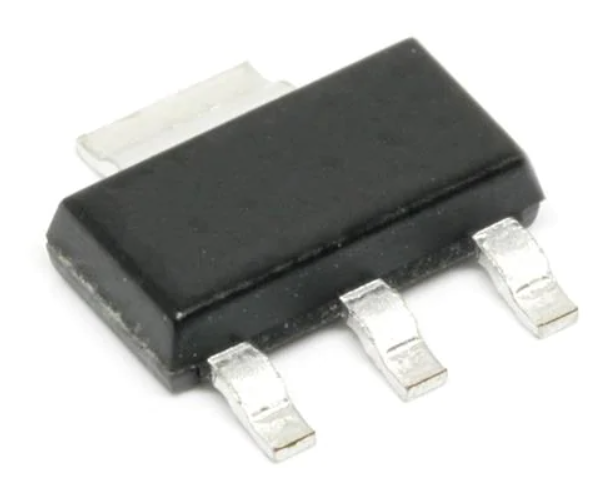
\includegraphics[width=0.20\linewidth]{Pictures/LT1117_AnalogD.png} 
  \caption{Circuito Integrado LT1117}
  \label{fig:LT1117_IC}
\end{figure}

La implementación del regulador lineal LT1117 es un proceso significativamente más simple. Es simplemente seguir el esquemático que se muestra en la Figura \ref{fig:Esquematico_LT1117_IC}.

\begin{figure}[h]
\centering
\includegraphics[width=0.42\linewidth]{Pictures/Esquemático LT1117_IC.png}
\caption{Esquemático del regulador lineal LT1117}
\label{fig:Esquematico_LT1117_IC}
\end{figure}


Para determinar los valores apropiados de resistencias, se utiliza la ecuación \ref{eq:tension_salida_LT1117}.

\begin{equation}\label{eq:tension_salida_LT1117}
V_{\text{out}} = 1.25 \, \text{V} \left(1 + \frac{R2}{R1}\right)
\end{equation}

Este enfoque simplificado facilita el diseño del regulador lineal LT1117. Ahora bien, para poder determinar la potencia disipada, Analog Devices en su hoja técnica brinda la ecuación \ref{eq:potencia_dissipada}.
\newpage
\begin{equation}
P_D = (V_{in} - V_{out}) \cdot I_{out}
\label{eq:potencia_dissipada}
\end{equation}


Donde:\\
$P_D$ es la potencia disipada.\\
$V_{in}$ es el voltaje de entrada.\\
$V_{out}$ es el voltaje de salida.\\
$I_{out}$ es la corriente de salida.

La eficiencia de un sistema (E) se define como la relación entre la potencia de salida ($P_{\text{out}}$) y la potencia de entrada ($P_{\text{in}}$), y se expresa en la ecuación \ref{eq:eficiencia}.

\begin{equation}
E = \frac{P_{\text{out}}}{P_{\text{in}}}
\label{eq:eficiencia}
\end{equation}

Donde, según la ecuación \ref{eq:potencia_dissipada}, la potencia de entrada ($P_{\text{in}}$) se calcula como:

\begin{equation}
P_{\text{in}} = (V_{\text{in}} - V_{\text{out}}) \cdot I_{\text{out}} + V_{\text{out}} \cdot I_{\text{out}}
\label{eq:eficiencia2}
\end{equation}

Y la potencia de salida ($P_{\text{out}}$) se calcula como:

\begin{equation}
P_{\text{out}} = V_{\text{out}} \cdot I_{\text{out}}
\label{eq:eficiencia3}
\end{equation}

Utilizando estas ecuaciones, podemos determinar la eficiencia porcentual de un regulador lineal como:

\begin{equation}
E (\%) = \frac{V_{\text{out}}}{V_{\text{in}}}\cdot 100\%.
\label{eq:eficiencia4}
\end{equation}

La eficiencia de la implementación de reguladores lineales se convierte en un tema preocupante cuando existe una diferencia significativa entre el voltaje de entrada y el de salida. \\\\Si consideramos las configuraciones previamente definidas (4s1p, 2s2p y 1s4p) para el banco de baterías, con voltajes nominales de entrada de 14.4 V, 7.2 V y 3.6 V respectivamente, podemos obtener resultados gráficos a partir de la ecuación \ref{eq:eficiencia4}, como se muestra en la Fig. \ref{fig:LDO_Efficiency}.

\newpage

\begin{figure}[h]
  \centering
  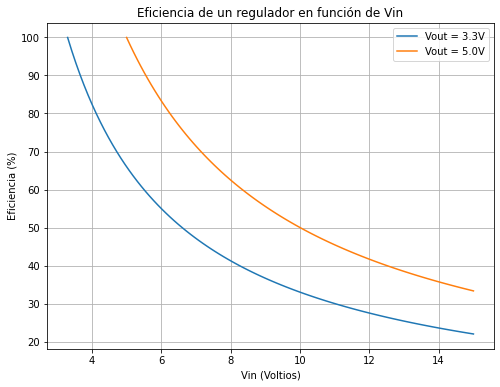
\includegraphics[width=0.8\linewidth]{Pictures/Grafica_Eficiencia_LDO.png} 
  \caption{Eficiencia del regulador LT1117 en función del voltaje de entrada ($V_{in}$)}
  \label{fig:LDO_Efficiency}
\end{figure}

Como resultado del análisis de la gráfica y considerando el contexto de diseño en el que se utilizaría el regulador de voltaje lineal LT1117, se concluye que su implementación no es conveniente. En el caso de la configuración 4s1p, la eficiencia es notablemente baja, siendo inferior al 35\% tanto para el bus de 3.3 V como para el de 5.0 V. Aunque la situación mejora ligeramente en la configuración 2s2p donde el vin es de 7.2 V, la eficiencia aún no alcanza ni siquiera el 70\%.

Finalmente, para el arreglo 1s4p donde el voltaje de entrada inicial sería 3.6 V se presenta un inconveniente inherente a los reguladores lineales, ya que no es posible construir un elevador de voltaje ('boost') con este dispositivo. Esto significa que no se podría obtener un bus de 5.0 V. Para el voltaje de 3.3 V, según la hoja de datos del fabricante \cite{analog_lt1117fd}, el voltaje de entrada mínimo necesario para regular y llevarlo a 3.3 V debe ser al menos de 5.0 V. \\\\Además, en el bus de 3.3 V precisamente se presenta un escenario aún más complejo, nos encontramos en una situación en la que el voltaje de la batería disminuiría hasta un valor de 2.5 V, lo que requeriría nuevamente una configuración 'boost'. Por lo tanto, debido a estas limitaciones y desafíos técnicos, se descarta el uso de reguladores lineales para esta aplicación.
\newpage

\textbf{MC34063A}

\begin{figure}[h]
  \centering
  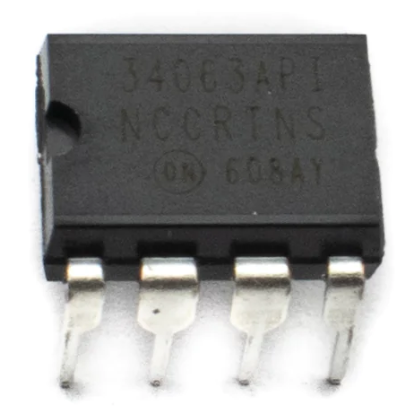
\includegraphics[width=0.25\linewidth]{Pictures/MC34063_IC.png} 
  \caption{Circuito Integrado MC34063A}
  \label{fig:MC34063_IC}
\end{figure}

Para la implementación del convertidor DC-DC MC34063, se emplean fórmulas esenciales proporcionadas por el fabricante y resumidas en la Tabla \ref{tab:forms_MC34063A} \cite{ti_mc34063a}. Adicionalmente, se utiliza una herramienta calculadora desarrollada por la comunidad de electrónicos para agilizar el proceso de diseño \cite{nomad_ee_mc34063a}. En cuanto al esquemático, se presenta la configuración Boost en la Figura \ref{fig:BoostMC} y la configuración Buck en la Figura \ref{fig:BuckMC}. La evaluación de la eficiencia se basa en tablas de referencia proporcionadas por el fabricante.

\begin{figure}[h]
  \centering
  \begin{subfigure}{0.4\linewidth}
    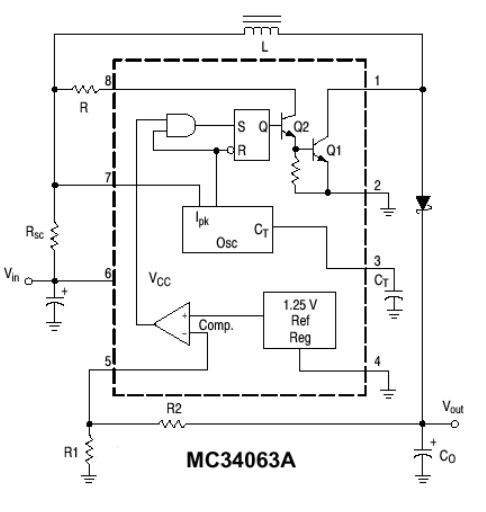
\includegraphics[width=\textwidth]{Pictures/Esquematico_Boost_Converter.png}
    \caption{MC34063A Configuración Boost}
    \label{fig:BoostMC}
  \end{subfigure}
  \begin{subfigure}{0.42\linewidth}
    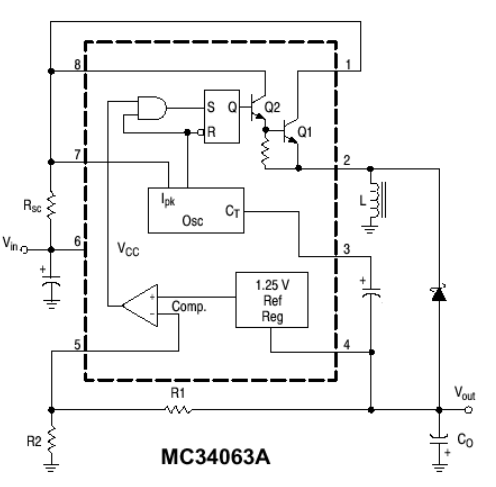
\includegraphics[width=\textwidth]{Pictures/Esquematico_Buck_Converter.png}
    \caption{MC34063A Configuración Buck}
    \label{fig:BuckMC}
  \end{subfigure}
  \caption{Configuraciones MC34063A}
\end{figure}

\begin{table}[!ht]
    \centering
    \renewcommand{\arraystretch}{2} % Espacio entre filas
    \begin{adjustbox}{max width=\textwidth}
        \begin{tabular}{ccc}
            \hline
            \makecell{Cálculo} & \makecell{Step-Up} & \makecell{Step-Down} \\
            \hline
            \makecell{$\frac{t_{on}}{t_{off}}$} & \makecell{$\frac{{V_{out} + V_F + V_{in(min)}}}{V_{in(min)}-V_{sat}}$} & \makecell{$\frac{V_{out} + V_F}{V_{in(min)}-V_{sat}-V_{out}}$} \\
            \hline
            \makecell{$t_{on}+{t_{off}}$} & \makecell{$\frac{1}{f}$} & \makecell{$\frac{1}{f}$} \\
            \hline
            \makecell{$t_{off}$} & \makecell{$\frac{t_{on}+t_{off}}{\frac{t_{on}}{t_{off}}+1}$} & \makecell{$\frac{t_{on}+t_{off}}{\frac{t_{on}}{t_{off}}+1}$} \\
            \hline
            \makecell{$t_{on}$}  & \makecell{$(t_{on}+{t_{off}})-{t_{off}}$} & \makecell{$(t_{on}+{t_{off}})-{t_{off}}$} \\
            \hline
            \makecell{$C_T$} & \makecell{$4.0x10^{-5}t_{on}$} & \makecell{$4.0x10^{-5}t_{on}$} \\
            \hline
            \makecell{$I_{pk(switch)}$} & \makecell{$2I_{out(max)}(\frac{t_{on}}{t_{off}}+1)$} & \makecell{$2I_{out(max)}$} \\
            \hline
            \makecell{$R_{sc}$} & \makecell{$\frac{0.3}{I_{pk(switch)}}$} & \makecell{$\frac{0.3}{I_{pk(switch)}}$} \\
            \hline
            \makecell{$L_(min)$} & \makecell{$(\frac{(V_{in(min)}-V_{sat})}{I_{pk(switch)}})t_{on(max)}$} & \makecell{$(\frac{(V_{in(min)}-V_{sat})}{I_{pk(switch)}})t_{on(max)}$} \\
            \hline
            \makecell{$C_O$} & \makecell{$9\frac{I_{out}I_{on}}{V_{ripple(pp)}}$} & \makecell{$\frac{I_{pk(switch)}(t_{on} + t_{off})}{8V_{ripple(pp)}}$} \\
            \hline
        \end{tabular}
    \end{adjustbox}
    \caption{Fórmulas de diseño para MC34063A}
    \label{tab:forms_MC34063A}
\end{table}

Un aspecto importante resaltado en la Tabla \ref{tab:forms_MC34063A} es el cálculo de la inductancia. El fabricante especifica un valor mínimo, lo que significa que al diseñar el circuito, existe flexibilidad para realizar ajustes finos según los resultados en la señal de salida o la disponibilidad de valores comerciales. Tanto el inductor como el condensador 'Co' forman un filtro pasabajos de segundo orden que desempeña un papel crucial en el convertidor DC-DC al reducir los sobreimpulsos antes de alcanzar el valor de estado estable.

Al igual que con el regulador de voltaje lineal LT1117, con el convertidor DC-DC evaluaremos el rendimiento con las configuraciones del banco de baterías 4s1p, 2s2p y 1s4p, previamente desarrolladas en las  \ref{fig:powerbank}, \ref{fig:powerbank2} y \ref{fig:powerbank3}.

Previo a desarrollar las simulaciones debemos recordar que en el capítulo de Requerimientos se realizó un presupuesto energético para cubrir la demanda de los subsistemas electrónicos de la misión StratoBalloon en Tabla \ref{tab:cuadro-cargas1} y \ref{tab:cuadro-cargas2}. 

En el presupuesto energético preliminar, no se consideraron las pérdidas asociadas a esta etapa de conversión de voltaje DC-DC, ni tampoco el autoconsumo de otros componentes relacionados con el Sistema de energía (EPS). Por lo tanto, al finalizar este capítulo, se llevará a cabo una revisión tomando estas consideraciones. Esto permitirá evaluar si el dimensionamiento del banco de baterías es adecuado. Dicho esto, iniciamos con la evaluación del convertidor para cada arreglo.

\newpage

%ARREGLO DE BATERÍAS 4S1P

\subsection{Arreglo de baterías 4s1p}

Como punto de partida consideramos el arreglo 4s1p. Para este arreglo, se toman en cuenta los valores detallados en la Tabla \ref{tab:valores_33_4s1p}

\begin{table*}[h]
    \centering
    \begin{tabular}{p{0.25\linewidth}p{0.1\linewidth}p{0.25\linewidth}p{0.1\linewidth}}
    \hline
    \textbf{Entradas} & \textbf{Valor} & \textbf{Salidas} & \textbf{Valor} \\ \hline
    Vin (min)[V] & 10.0 & Ct [pF] & 157 \\
    Vout [V] & 3.3 & Ipk [mA] & 1500 \\
    Iout [mA] & 750 & Rsc [Ohm] & 0.2 \\
    V ripple pp [mV] & 10 & Lmin [uH] & 15 \\
    Fmin [kHz] & 100 & Co [uF] & 188 \\
    ~ & ~ & R1 [kohm] & 11 \\
    ~ & ~ & R2 [kohm] & 18 \\ \hline
    \end{tabular}
\caption{Valores para convertidor DC-DC MC34063A, bus 3.3 V a 750 mA.}
\label{tab:valores_33_4s1p}
\end{table*}

Como resultado obtenemos la señal de voltaje de salida para el arreglo de baterías 4s1p a máxima carga en Fig. \ref{fig:4s1p_33v_2dcdcconverters_Max} y para mínima carga en Fig. \ref{fig:4s1p_33v_2dcdcconverters_min}.

\begin{figure}[h]
  \centering
  \begin{subfigure}{0.48\linewidth}
    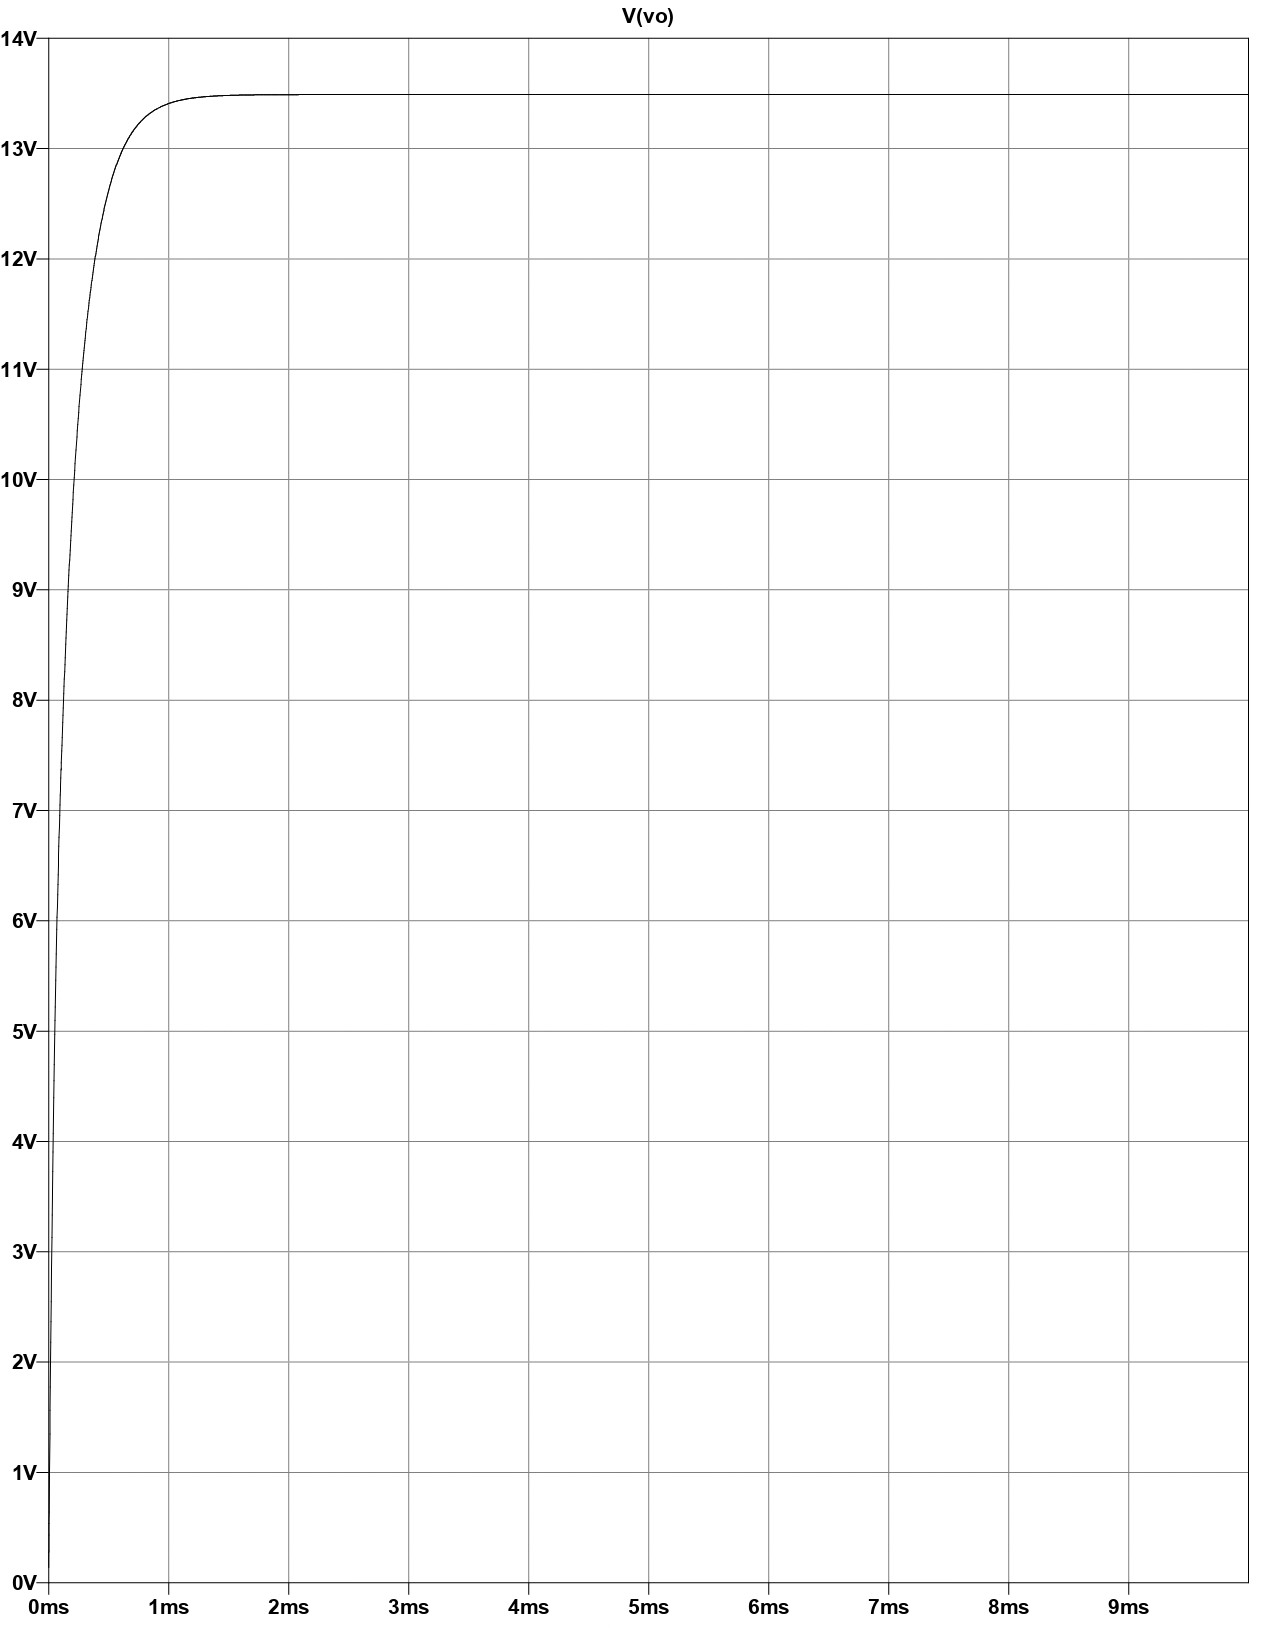
\includegraphics[width=\textwidth]{Pictures/Convertidor DC-DC MC34063A, bus 3.3 v a 750 mA_page-0001.jpg}
    \caption{Salida de voltaje a 3.3 voltios. Vin máximo (16.8 V)}
    \label{fig:4s1p_33v_2dcdcconverters_Max}
  \end{subfigure}
  \hfill
  \begin{subfigure}{0.48\linewidth}
    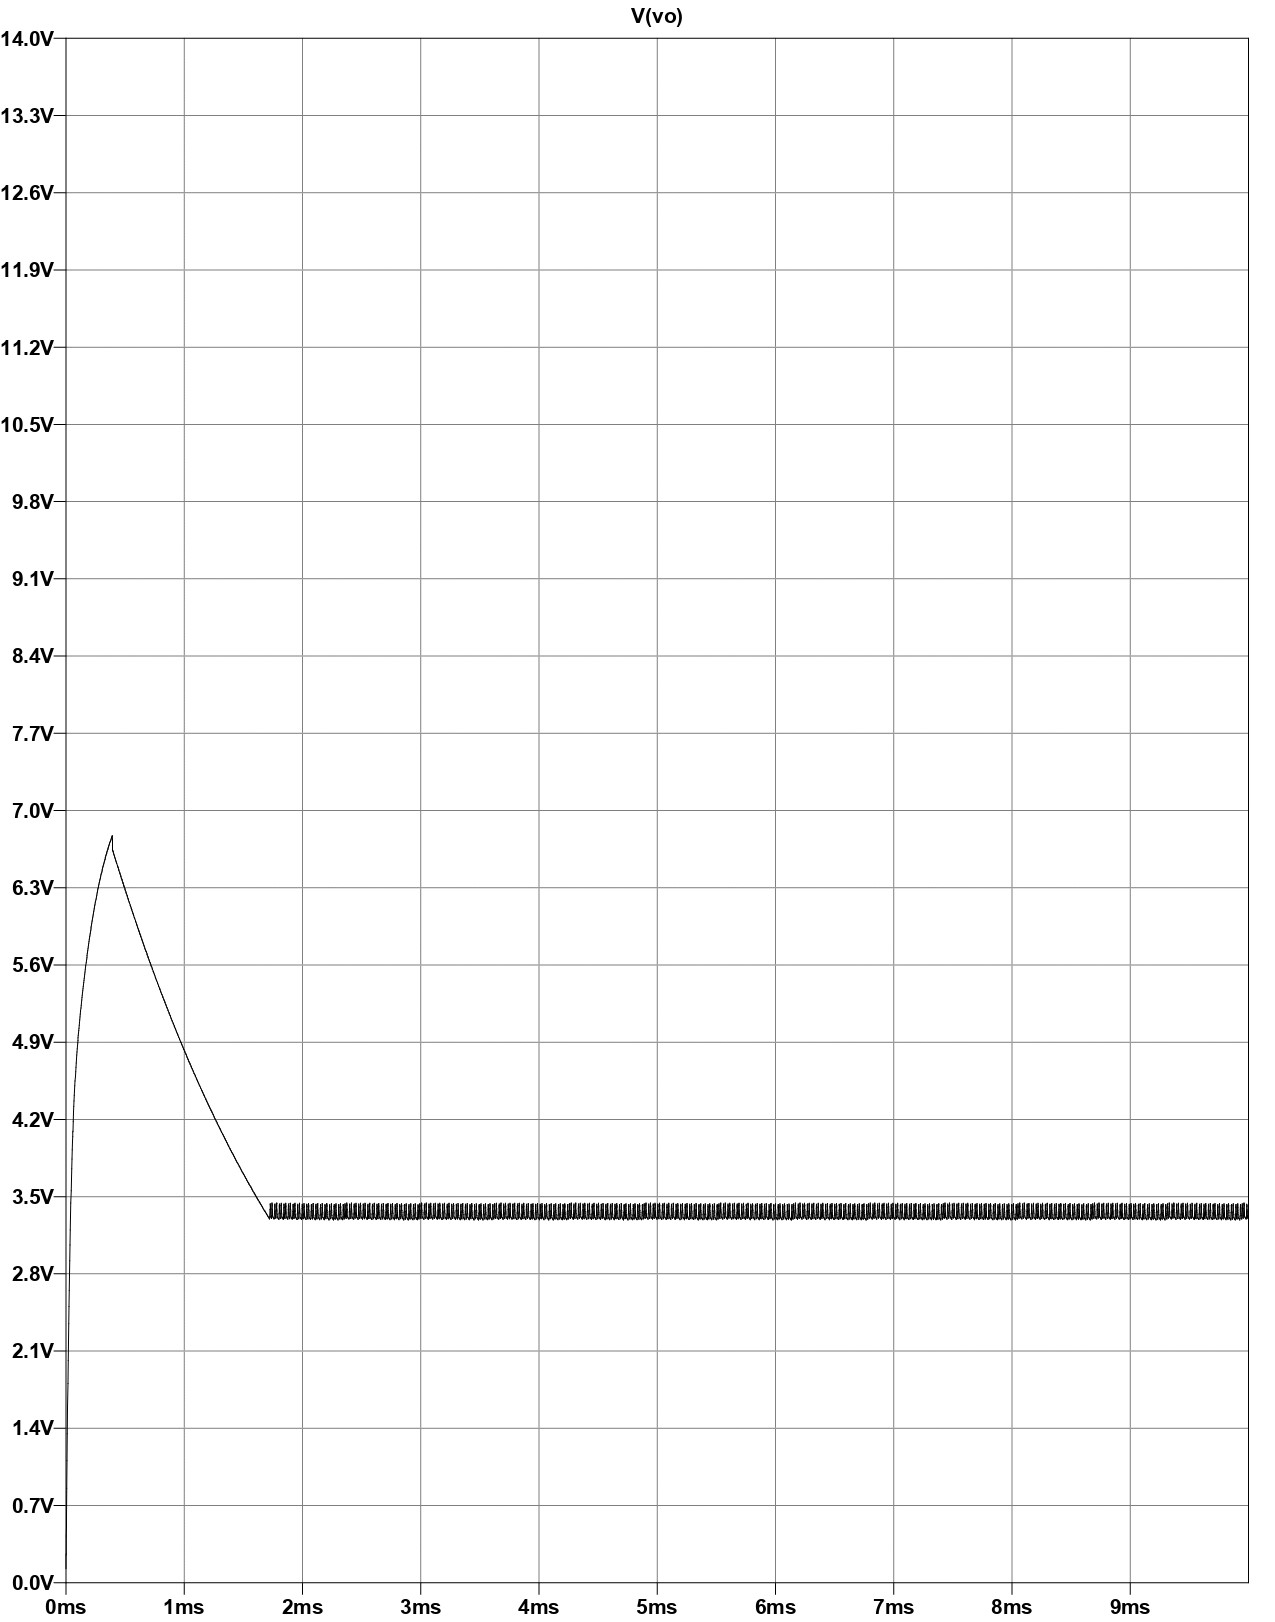
\includegraphics[width=\textwidth]{Pictures/Convertidor DC-DC MC34063A, bus 3.3 v a 750 mA_page-0001 Min.jpg}
    \caption{Salida de voltaje a 3.3 voltios. Vin mínimo. (10.0 V)}
    \label{fig:4s1p_33v_2dcdcconverters_min}
  \end{subfigure}
  \caption{Convertidor DC-DC MC34063A, arreglo 4s1p, bus de 3.3 V a 750 mA.}
  \label{fig:ConveridorDCDC_4S1P_33V}
\end{figure}

En el primer escenario (Fig. \ref{fig:4s1p_33v_2dcdcconverters_Max}), con las baterías completamente cargadas, observamos que el convertidor DC-DC no alcanza el valor de voltaje regulado.

En el escenario opuesto (Fig. \ref{fig:ConveridorDCDC_4S1P_33V}), con las baterías descargadas al mínimo, logramos alcanzar el valor deseado en estado estable. Sin embargo, se produce un sobreimpulso que alcanza hasta 6.3V, lo que representa un riesgo para los dispositivos electrónicos alimentados. La estabilización en 3.3V en este caso requiere aproximadamente 1.8 milisegundos. Por lo tanto, será necesario realizar un ajuste en el valor de la inductancia del circuito LC del convertidor.

Al ajustar los valores de la inductancia mínima a 30uH, obtenemos los resultados de la Fig. \ref{fig:ConveridorDCDC_4S1P_33V_ajustada}


\begin{figure}[h]
  \centering
  \begin{subfigure}{0.48\linewidth}
    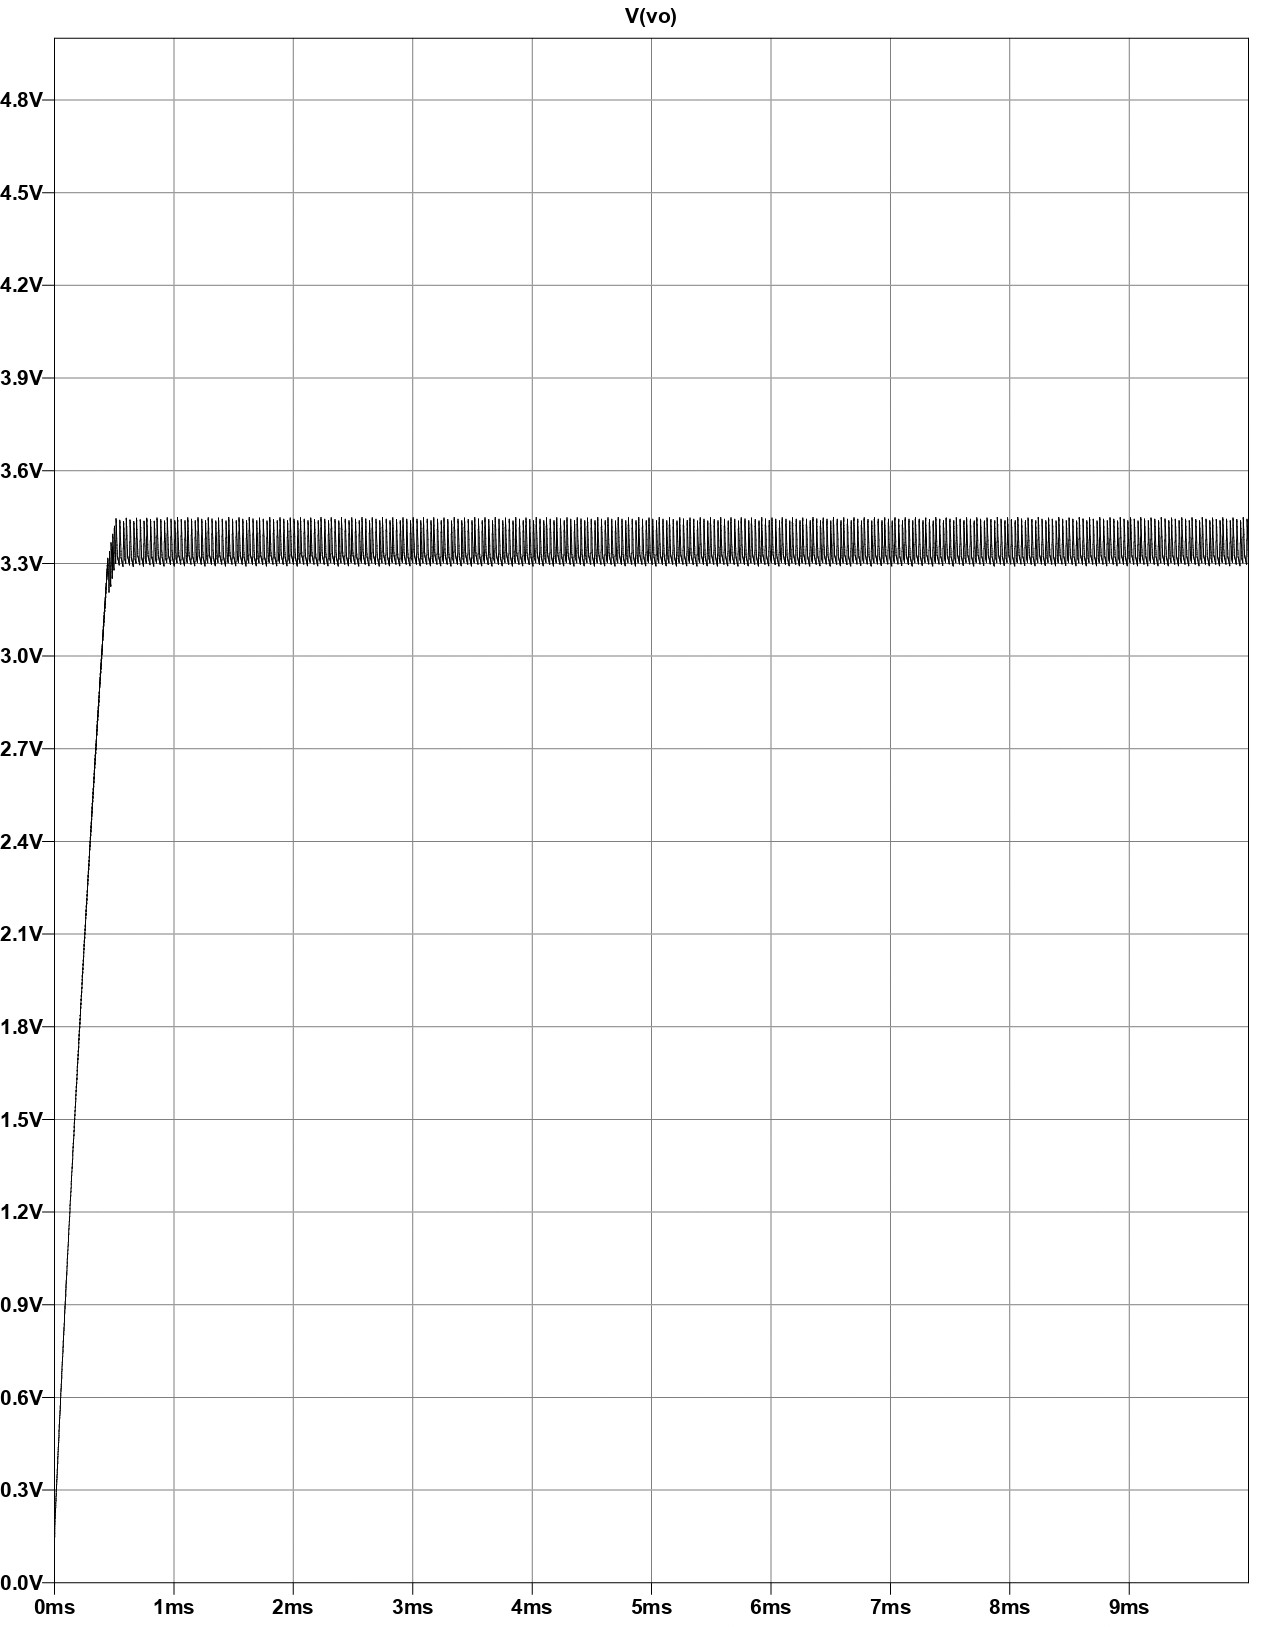
\includegraphics[width=\textwidth]{Pictures/Ajustada1_Max.jpg}
    \caption{Salida de voltaje a 3.3 voltios. Vin máximo (16.8 V). Inductancia ajustada a 30 uH.}
    \label{fig:4s1p_33v_2dcdcconverters_Max2}
  \end{subfigure}
  \hfill
  \begin{subfigure}{0.48\linewidth}
    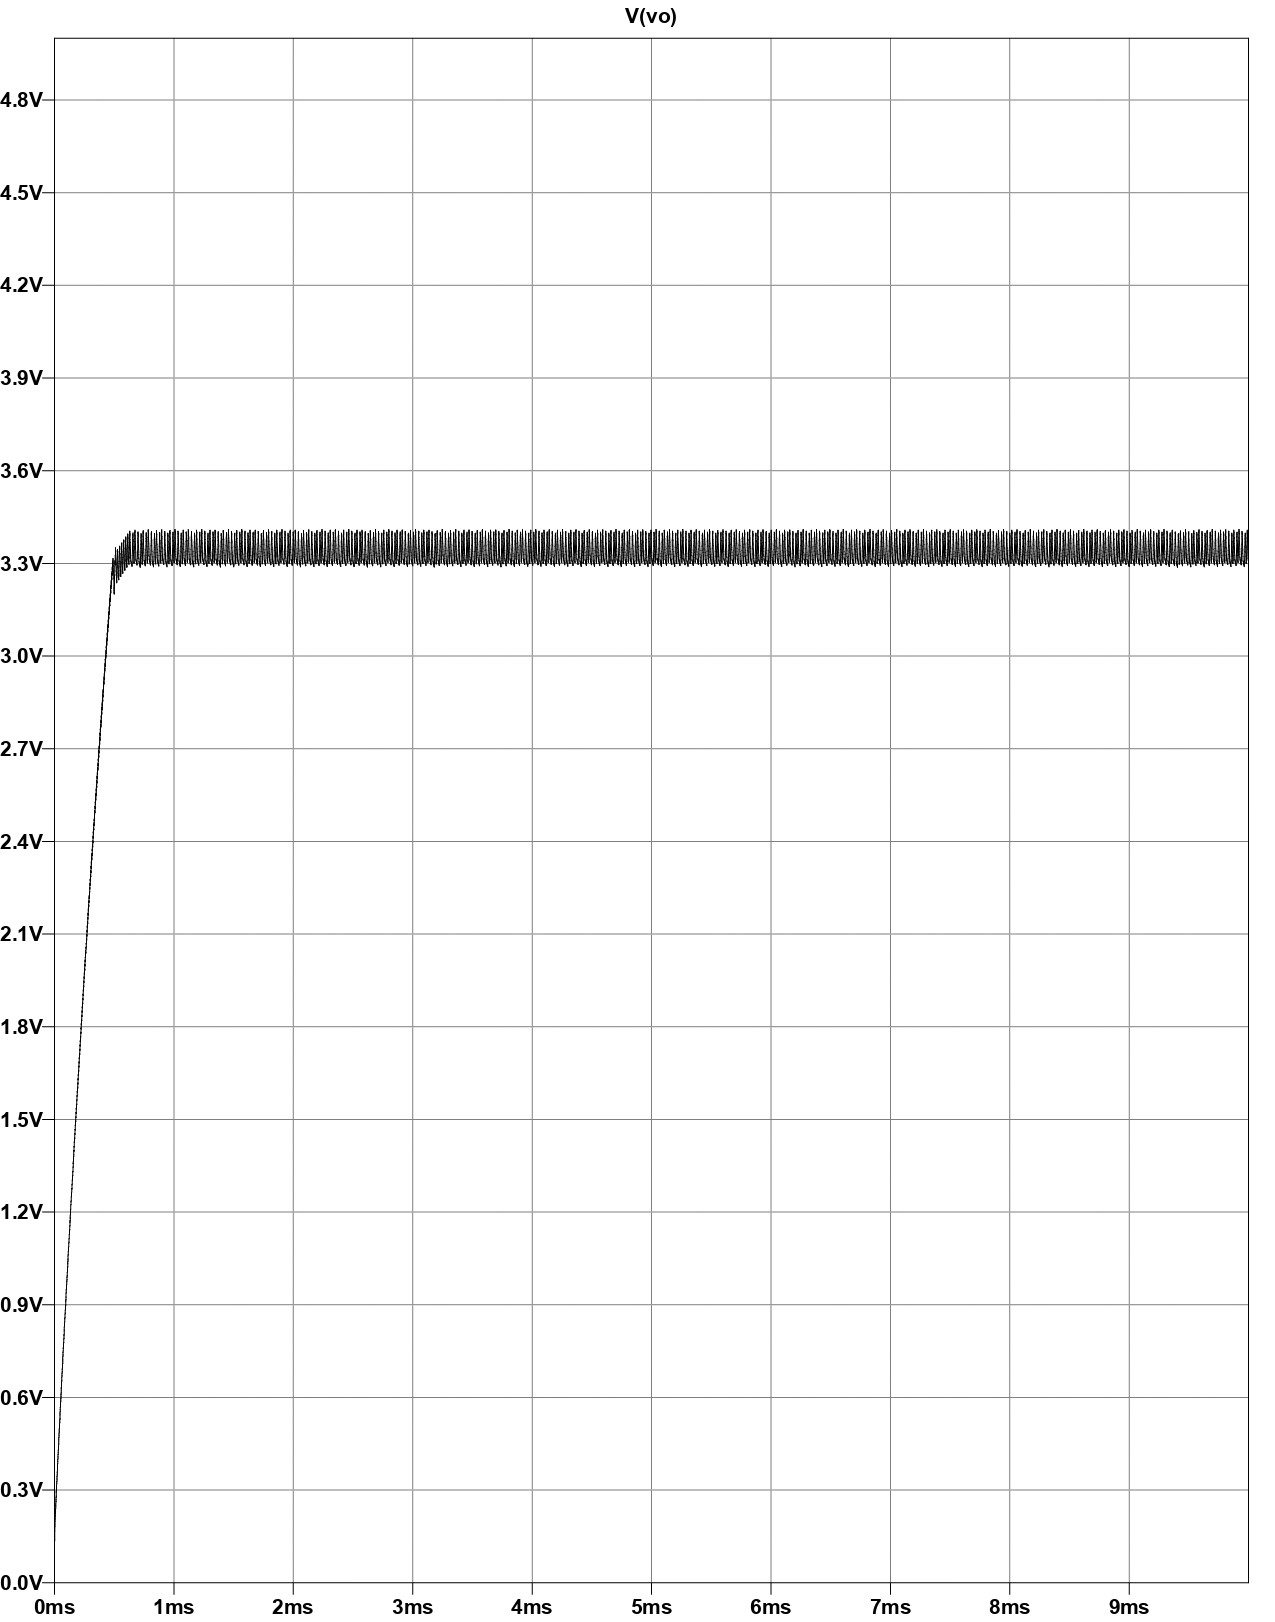
\includegraphics[width=\textwidth]{Pictures/Ajustada1_Min.jpg}
    \caption{Salida de voltaje a 3.3 voltios. Vin mínimo. (10.0 V). Inductancia ajustada a 30 uH.}
    \label{fig:4s1p_33v_2dcdcconverters_min2}
  \end{subfigure}
  \caption{Convertidor DC-DC MC34063A, arreglo 4s1p, bus de 3.3 V a 750 mA. Inductancia ajustada a 30 uH.}
  \label{fig:ConveridorDCDC_4S1P_33V_ajustada}
\end{figure}

Podemos observar que en ambos casos, los resultados son satisfactorios para alimentar las cargas. Tanto el valor pico a pico como el sobreimpulso se encuentran en niveles despreciables, lo que representa un resultado satisfactorio tanto en el caso del banco de baterías a máxima carga (ver Fig. \ref{fig:4s1p_33v_2dcdcconverters_Max2}) como en el caso de mínima carga (ver Fig. \ref{fig:ConveridorDCDC_4S1P_33V_ajustada}).

\newpage

% PARA EL BUS DE 5.0 VOLTIOS ************

Siguiendo un procedimiento similar, empleando los datos de la Tabla \ref{tab:valores_50_4s1p}, obtenemos los resultados para el voltaje máximo del banco de baterías en configuración 4s1p en Fig. \ref{fig:4s1p_50v_2dcdcconverters_Max} y el mínimo en Fig. \ref{fig:4s1p_50v_2dcdcconverters_min}.

\begin{table*}[h]
    \centering
    \begin{tabular}{p{0.25\linewidth}p{0.1\linewidth}p{0.25\linewidth}p{0.1\linewidth}}
    \hline
    \textbf{Entradas} & \textbf{Valor} & \textbf{Salidas} & \textbf{Valor} \\ \hline
    Vin (min)[V] & 10.0 & Ct [pF] & 230 \\
    Vout [V] & 5.0 & Ipk [mA] & 1500 \\
    Iout [mA] & 750 & Rsc [Ohm] & 0.2 \\
    V ripple pp [mV] & 10 & Lmin [uH] & 15 \\
    Fmin [kHz] & 100 & Co [uF] & 188 \\
    ~ & ~ & R1 [kohm] & 1 \\
    ~ & ~ & R2 [kohm] & 3 \\ \hline
    \end{tabular}
\caption{Valores para convertidor DC-DC MC34063A, arreglo 4s1p, bus 5.0 V a 750 mA.}
\label{tab:valores_50_4s1p}
\end{table*}


\begin{figure}[h]
  \centering
  \begin{subfigure}{0.48\linewidth}
    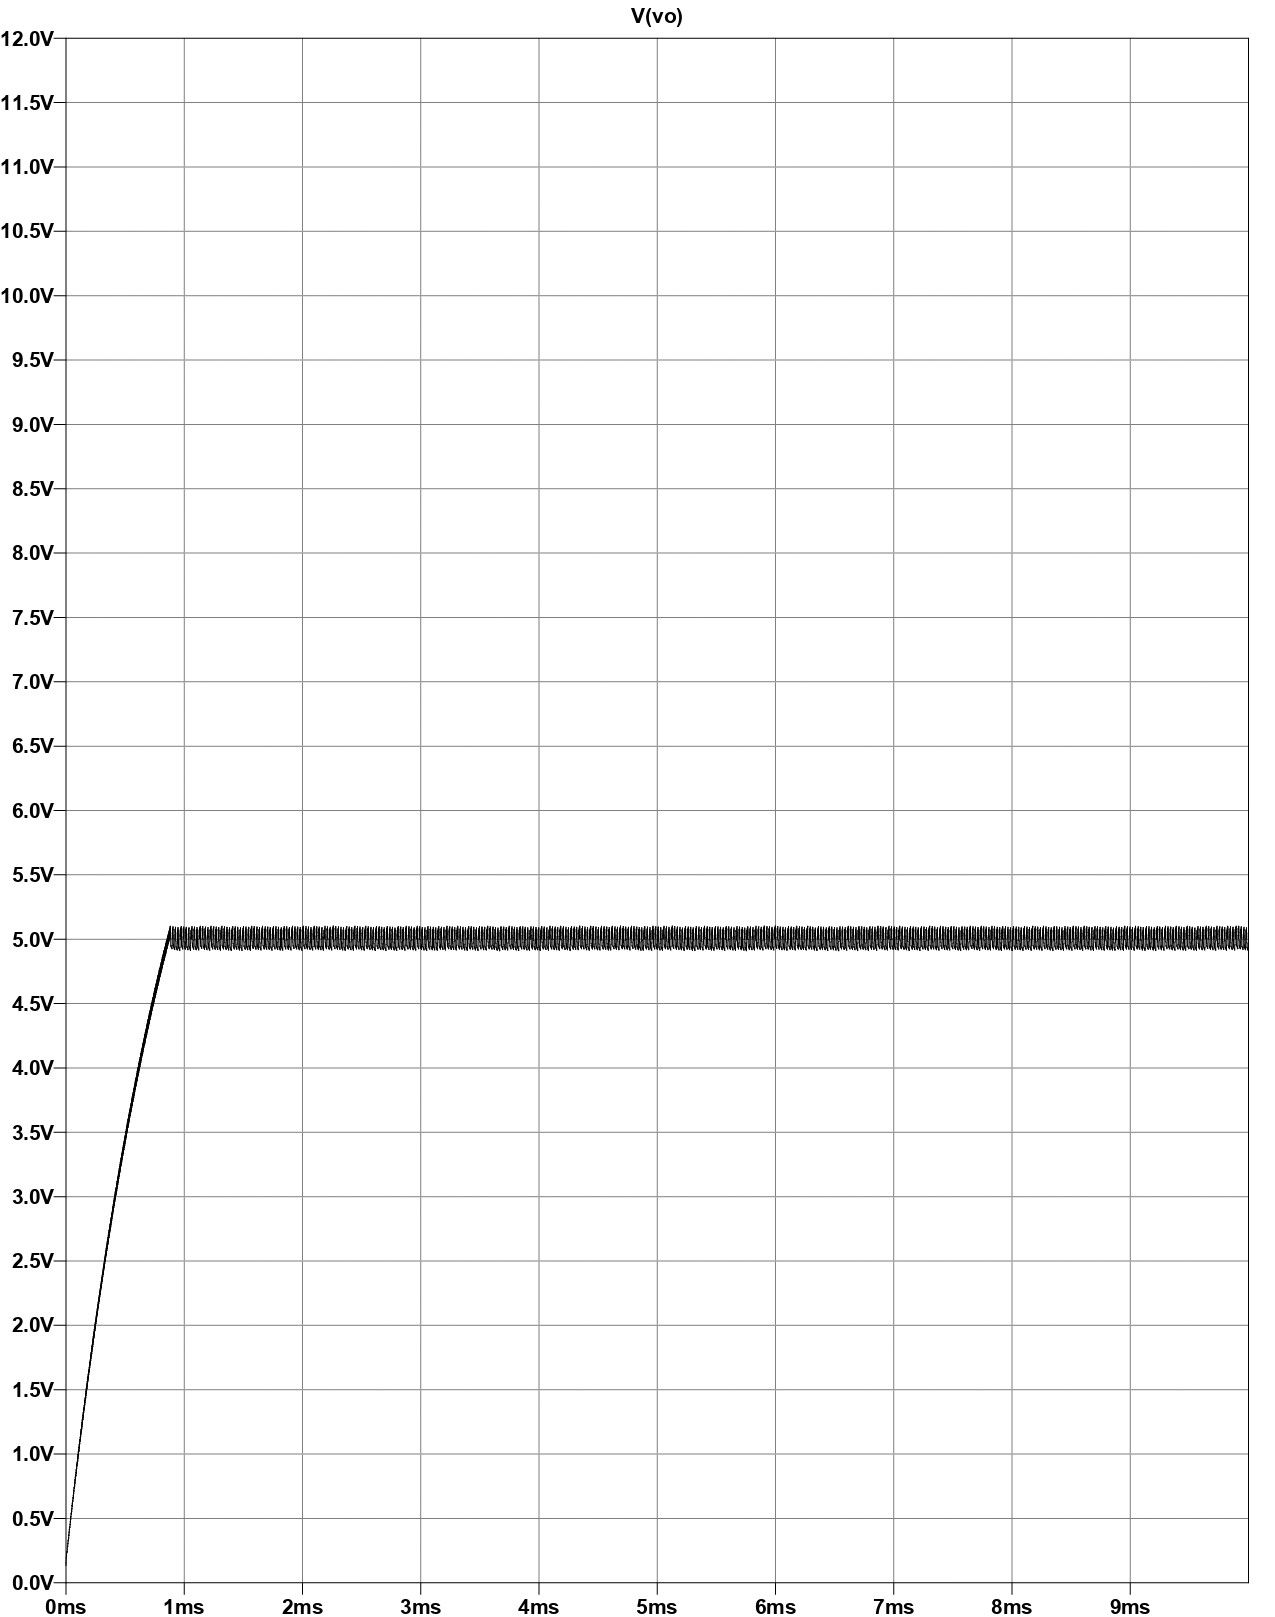
\includegraphics[width=\textwidth]{Pictures/Convertidor DC-DC MC34063A, bus 5.0 v a 750 mA_page-0001 Max.jpg}
    \caption{Salida de voltaje a 5.0 voltios. Vin máximo (16.8 V)}
    \label{fig:4s1p_50v_2dcdcconverters_Max}
  \end{subfigure}
  \hfill
  \begin{subfigure}{0.48\linewidth}
    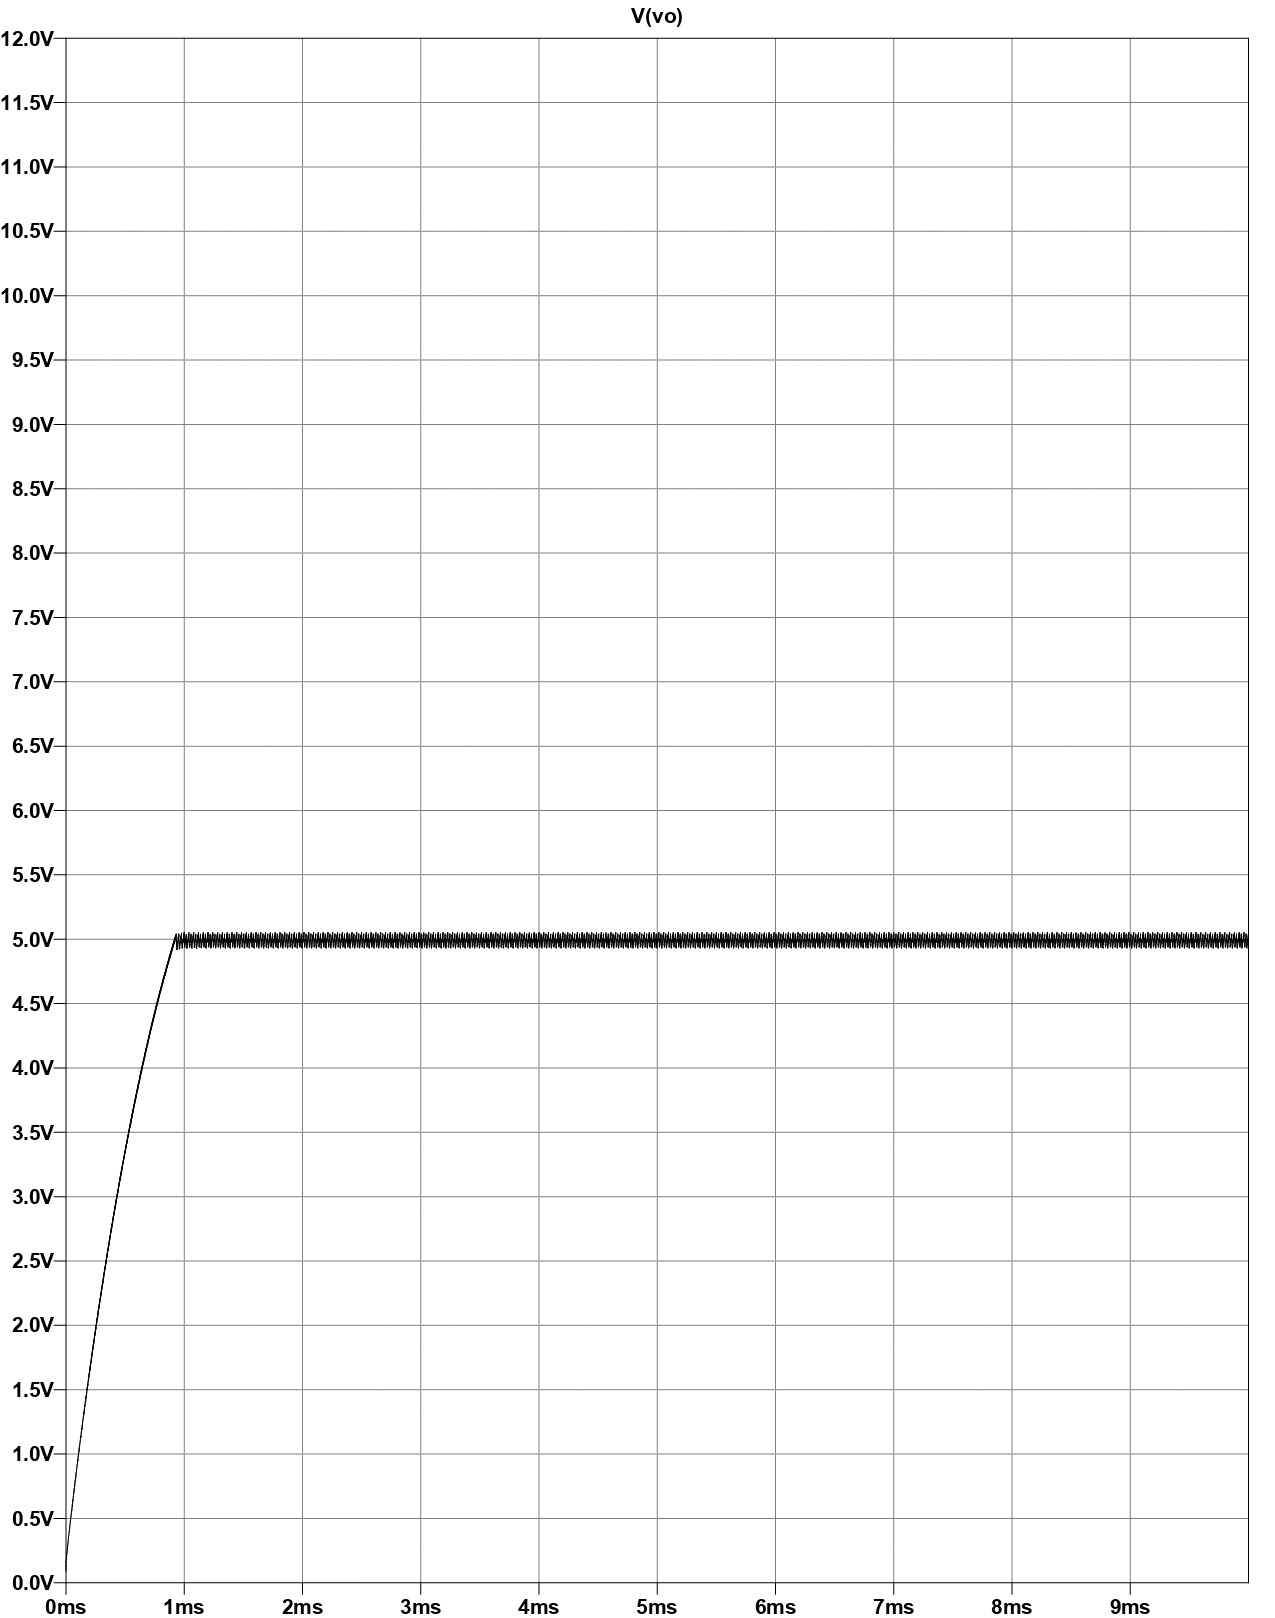
\includegraphics[width=\textwidth]{Pictures/Convertidor DC-DC MC34063A, bus 5.0 v a 750 mA_page-0001 Min.jpg}
    \caption{Salida de voltaje a 5.0 voltios. Vin mínimo. (10.0 V)}
    \label{fig:4s1p_50v_2dcdcconverters_min}
  \end{subfigure}
  \caption{Convertidor DC-DC MC34063A, arreglo 4s1p, bus de 5.0 V a 750 mA.}
\end{figure}

Podemos observar que en ambos casos, los resultados son satisfactorios para alimentar las cargas. Tanto el valor pico a pico como el sobreimpulso se encuentran en niveles despreciables, lo que representa un resultado satisfactorio sin requerir el ajuste de la inductancia del filtro pasabajos.




% ARREGLO 2S2P
\subsection{Arreglo de baterías 2s2p}
Como segundo arreglo del banco de baterías consideramos la configuración 2s2p. Empleamos los cálculos de la Fig. \ref{tab:valores_33_2s2p} y como resultado se obtiene la Fig. \ref{fig:2s2p_33v_2dcdcconverters_Max} para un banco de baterías con carga máxima y la Fig. \ref{fig:2s2p_33v_2dcdcconverters_min} para carga al mínimo.

% PARA EL BUS DE 3.3 VOLTIOS ************

\begin{table*}[h]
    \centering
    \begin{tabular}{p{0.25\linewidth}p{0.1\linewidth}p{0.25\linewidth}p{0.1\linewidth}}
    \hline
    \textbf{Entradas} & \textbf{Valor} & \textbf{Salidas} & \textbf{Valor} \\ \hline
    Vin (min)[V] & 5.0 & Ct [pF] & 336 \\
    Vout [V] & 3.3 & Ipk [mA] & 1500 \\
    Iout [mA] & 750 & Rsc [Ohm] & 0.2 \\
    V ripple pp [mV] & 10 & Lmin [uH] & 4 \\
    Fmin [kHz] & 100 & Co [uF] & 188 \\
    ~ & ~ & R1 [kohm] & 11 \\
    ~ & ~ & R2 [kohm] & 18 \\ \hline
    \end{tabular}
\caption{Valores para convertidor DC-DC MC34063A, arreglo 2s2p, bus 3.3 V a 750 mA.}
\label{tab:valores_33_2s2p}
\end{table*}


\begin{figure}[h]
  \centering
  \begin{subfigure}{0.48\linewidth}
    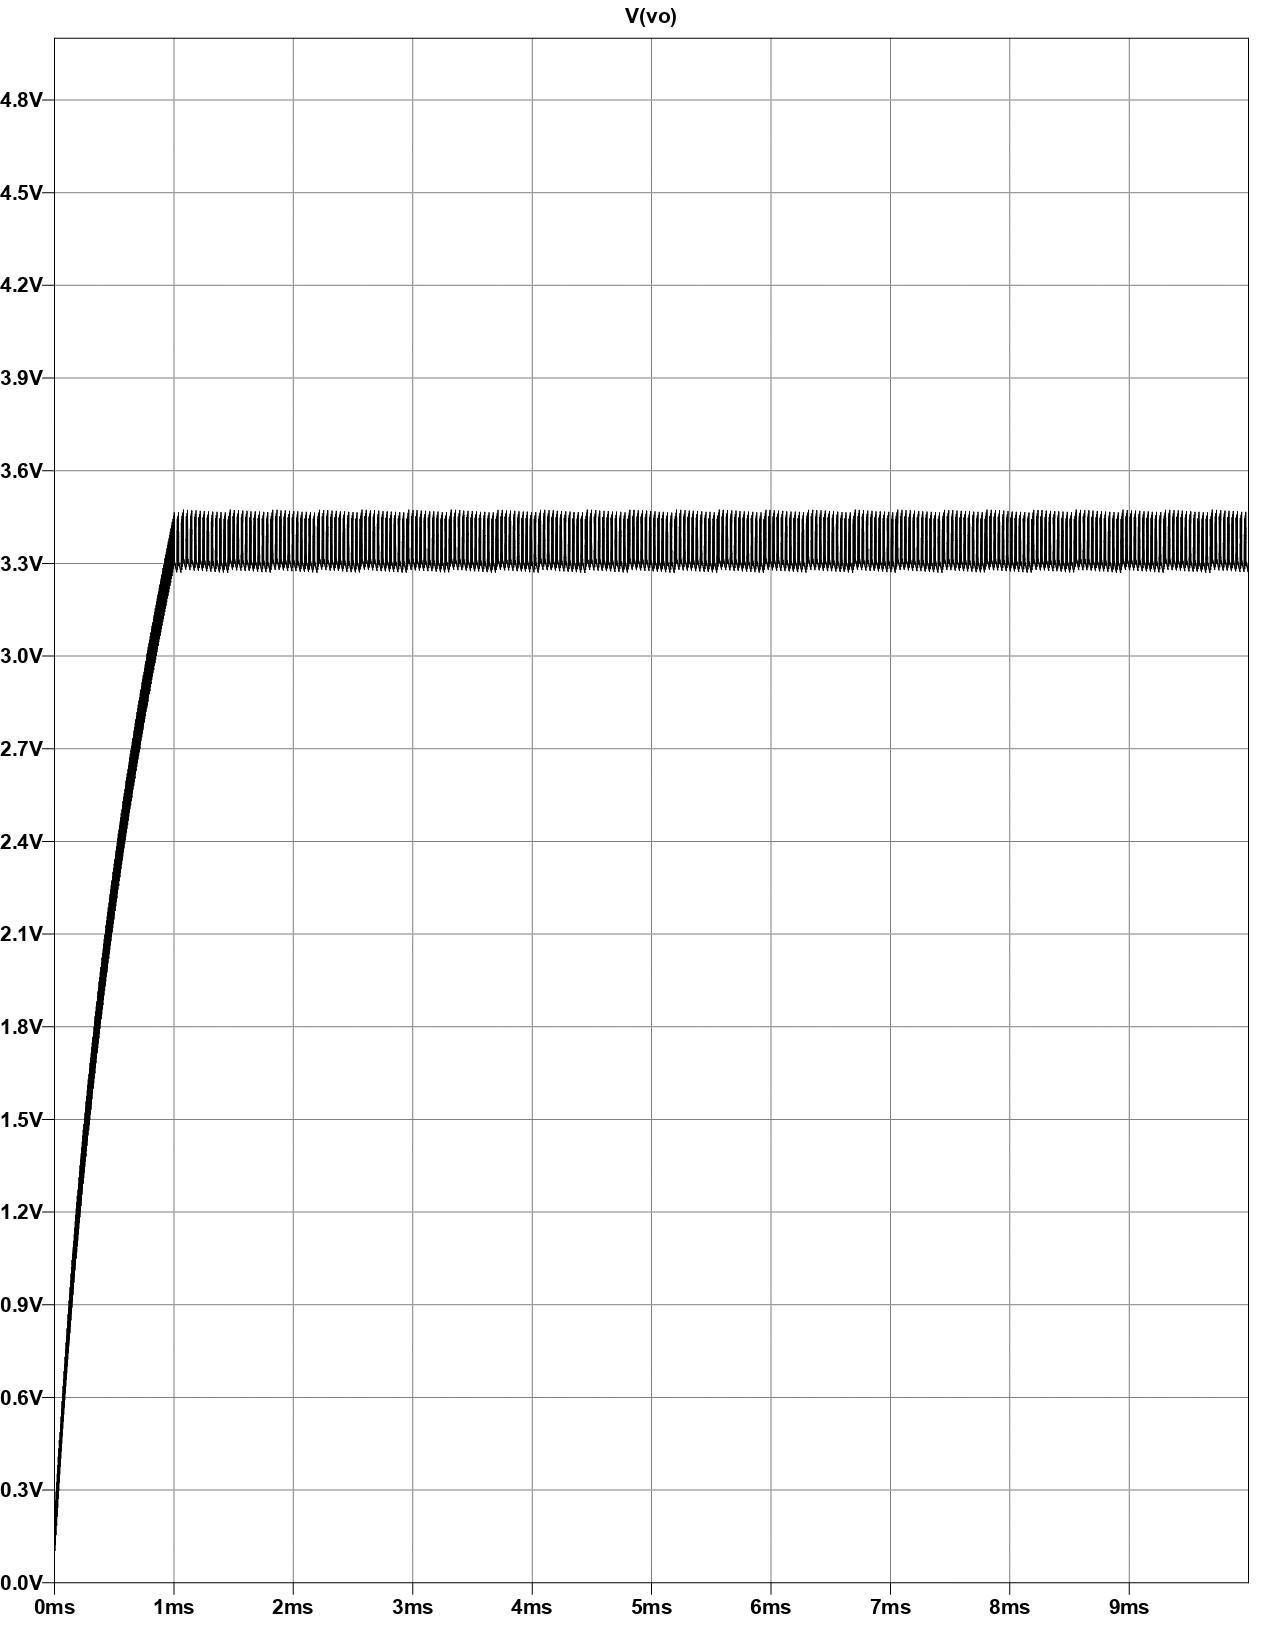
\includegraphics[width=\textwidth]{Pictures/Convertidor DC-DC MC34063A, 2s2p, bus 3.3 v a 750 mA_page-0001 Max.jpg}
    \caption{Salida de voltaje a 3.3 voltios. Vin máximo (8.4 V).}
    \label{fig:2s2p_33v_2dcdcconverters_Max}
  \end{subfigure}
  \hfill
  \begin{subfigure}{0.48\linewidth}
    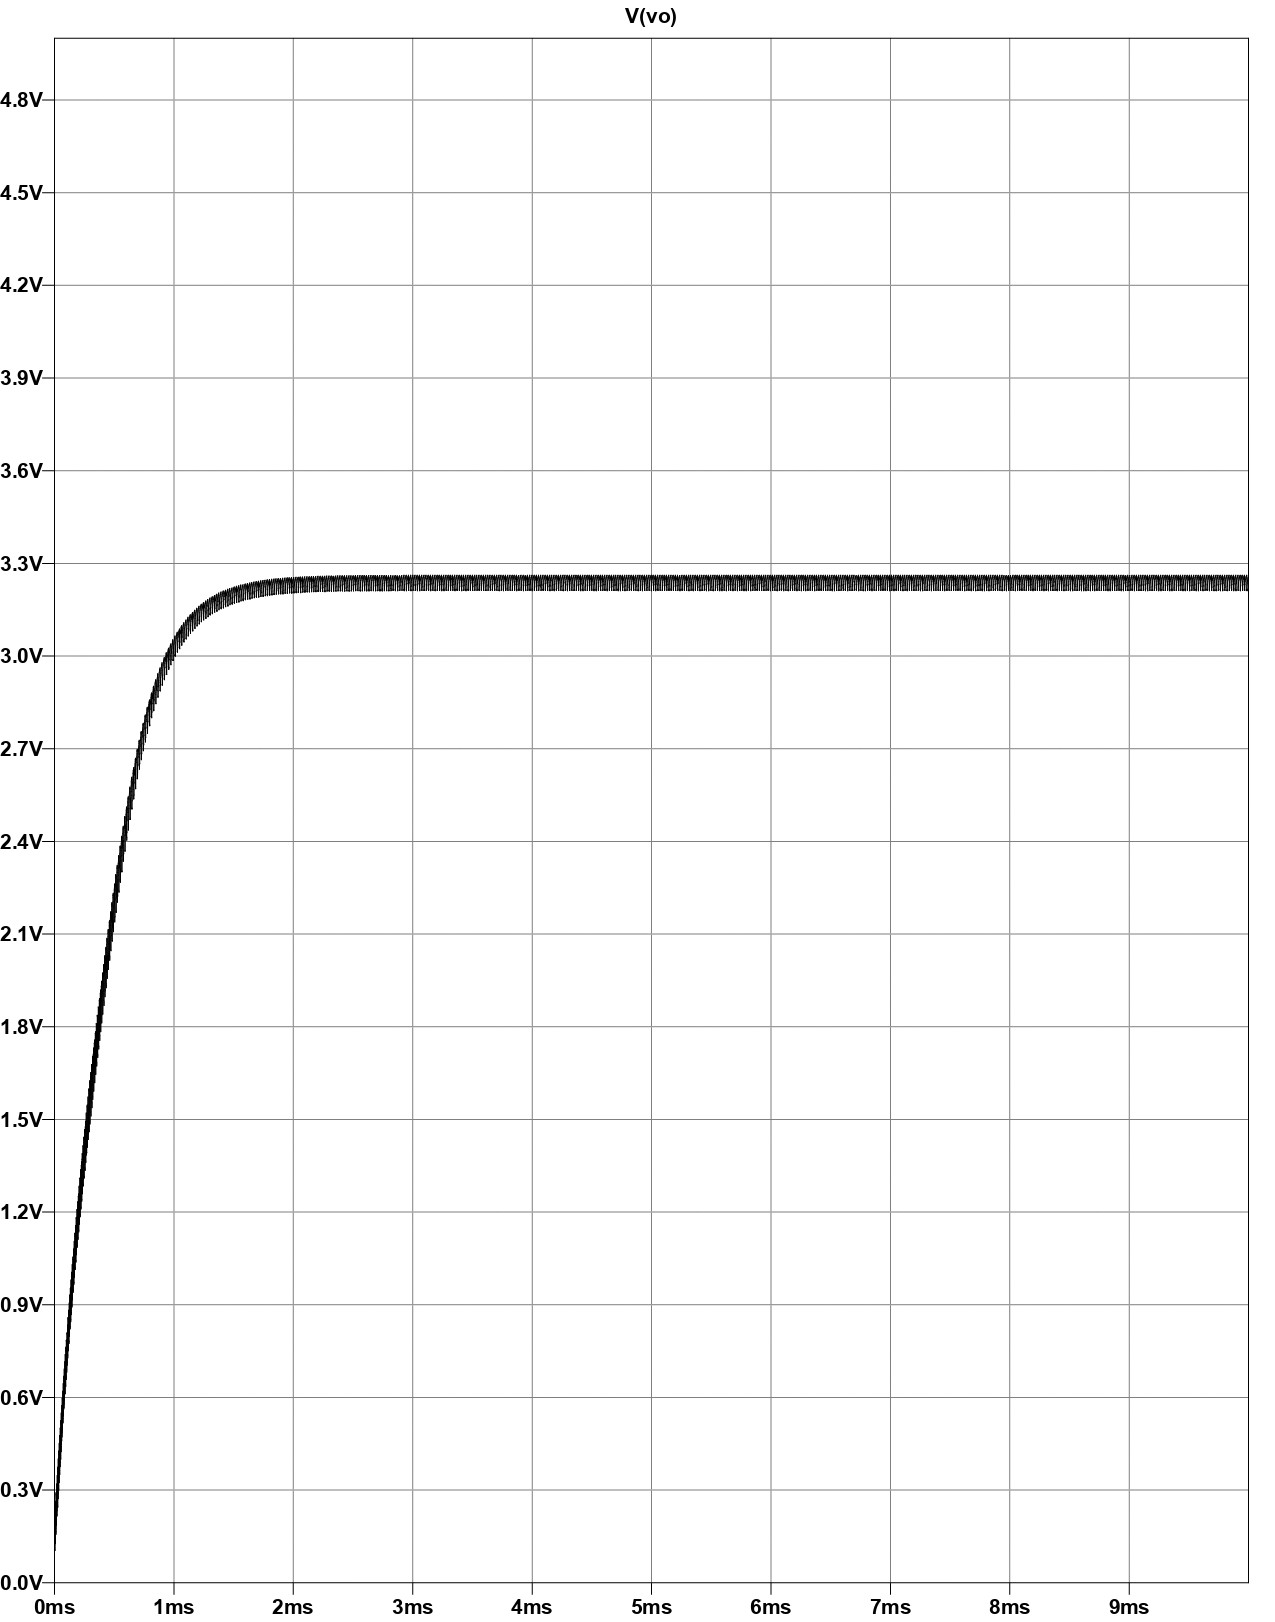
\includegraphics[width=\textwidth]{Pictures/Convertidor DC-DC MC34063A, 2s2p, bus 3.3 v a 750 mA_page-0001 Min.jpg}
    \caption{Salida de voltaje a 3.3 voltios. Vin mínimo operativo (5.5 V).}
    \label{fig:2s2p_33v_2dcdcconverters_min}
  \end{subfigure}
  \caption{Convertidor DC-DC MC34063A, arreglo 2s2p, bus de 3.3 V a 750 mA.}
\end{figure}

\newpage

Podemos observar que en ambos casos, los resultados son satisfactorios para alimentar las cargas. Tanto el valor pico a pico como el sobreimpulso se encuentran en niveles tolerables, lo que representa un resultado satisfactorio sin requerir el ajuste de la inductancia del filtro pasabajos.

Es importante mencionar que en el caso de la Figura \ref{fig:2s2p_33v_2dcdcconverters_min}, se considera como valor mínimo operativo 5.5V, ya que según simulaciones, este es el valor mínimo que el banco de baterías puede proporcionar para obtener una salida regulada de 3.3V. Sin embargo, según la hoja técnica del fabricante y la curva de descarga del modelo de batería Panasonic 18650b, esto se considera despreciable en términos de carga almacenada \cite{panasonic_18650b}.

% PARA EL BUS DE 5.0 VOLTIOS ************

Siguiendo un procedimiento similar, empleamos los cálculos de la Tabla \ref{tab:valores_50_2s2p}, y obtenemos los resultados de la Fig. \ref{fig:2s2p_50v_2dcdcconverters_Max} para un banco de baterías a máxima carga y la Fig. \ref{fig:2s2p_50v_2dcdcconverters_min} a mínima carga.

\begin{table*}[h]
    \centering
    \begin{tabular}{p{0.25\linewidth}p{0.1\linewidth}p{0.25\linewidth}p{0.1\linewidth}}
    \hline
    \textbf{Entradas} & \textbf{Valor} & \textbf{Salidas} & \textbf{Valor} \\ \hline
    Vin (min)[V] & 5.5 & Ct [pF] & 327 \\
    Vout [V] & 5.0 & Ipk [mA] & 1500 \\
    Iout [mA] & 500 & Rsc [Ohm] & 0.3 \\
    V ripple pp [mV] & 10 & Lmin [uH] & 10 \\
    Fmin [kHz] & 100 & Co [uF] & 125 \\
    ~ & ~ & R1 [kohm] & 1 \\
    ~ & ~ & R2 [kohm] & 3 \\ \hline
    \end{tabular}
\caption{Valores para convertidor DC-DC MC34063A, arreglo 2s2p, bus 5.0 V a 750 mA.}
\label{tab:valores_50_2s2p}
\end{table*}

Al analizar los resultados presentados en la Figura \ref{fig:arreglo2s2p5vdc}, se aprecia que en condiciones de máxima carga (Fig. \ref{fig:2s2p_50v_2dcdcconverters_Max}), no se logra alcanzar el voltaje deseado para la regulación, y esta situación se agrava en condiciones de mínima carga en el banco de baterías (Fig. \ref{fig:2s2p_50v_2dcdcconverters_min}). Esta discrepancia puede atribuirse a la diferencia entre el voltaje de entrada y el voltaje objetivo en este arreglo para el convertidor DC-DC .

Aunque en esta ocasión no se observan problemas relacionados con sobreimpulsos, este diseño no se considera adecuado para aplicaciones del EPS debido a que los valores de tensión necesarios no se alcanzan y, en consecuencia, los componentes electrónicos no funcionarían de manera óptima.


\begin{figure}[h]
  \centering
  \begin{subfigure}{0.48\linewidth}
    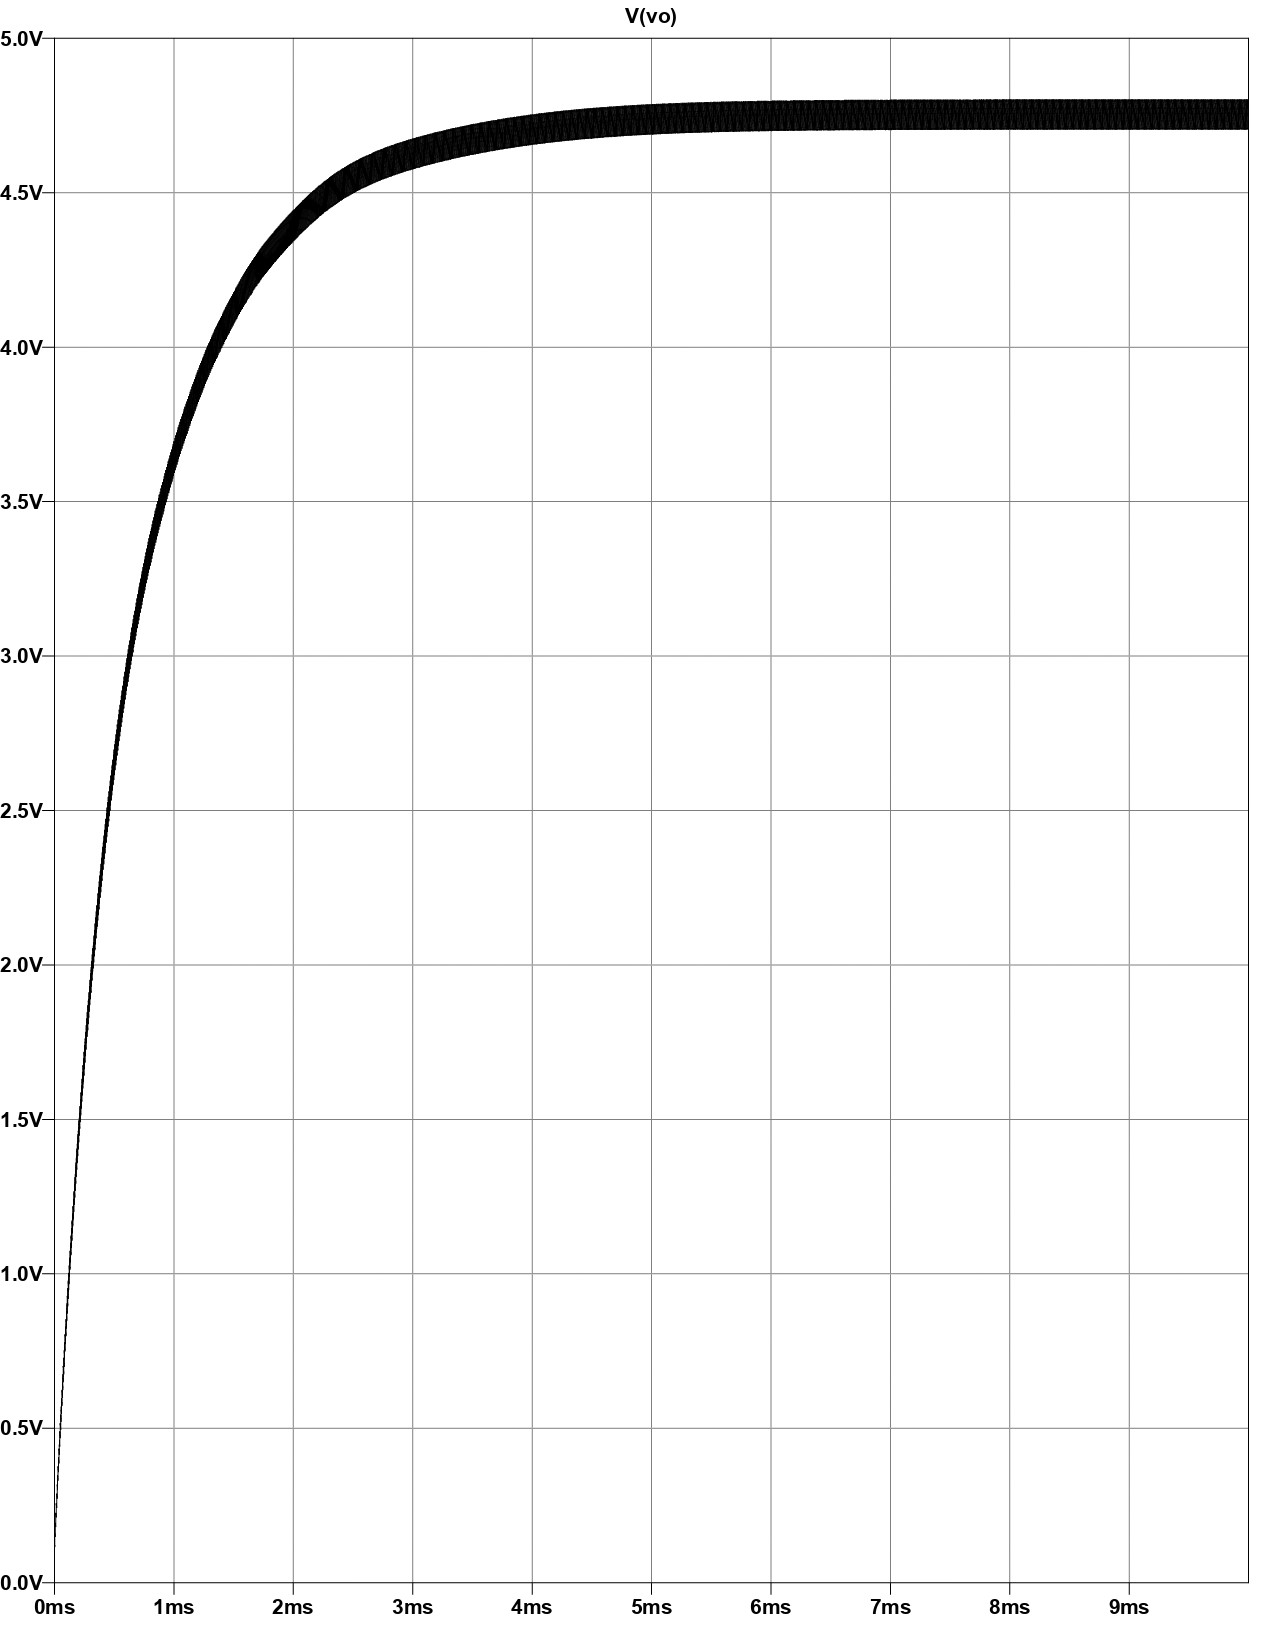
\includegraphics[width=\textwidth]{Pictures/Convertidor DC-DC MC34063A, 2s2p, bus 5.0 v a 500 mA_page-0001 Max.jpg}
    \caption{Salida de voltaje a 5.0 voltios. Vin máximo (8.4 V).}
    \label{fig:2s2p_50v_2dcdcconverters_Max}
  \end{subfigure}
  \hfill
  \begin{subfigure}{0.48\linewidth}
    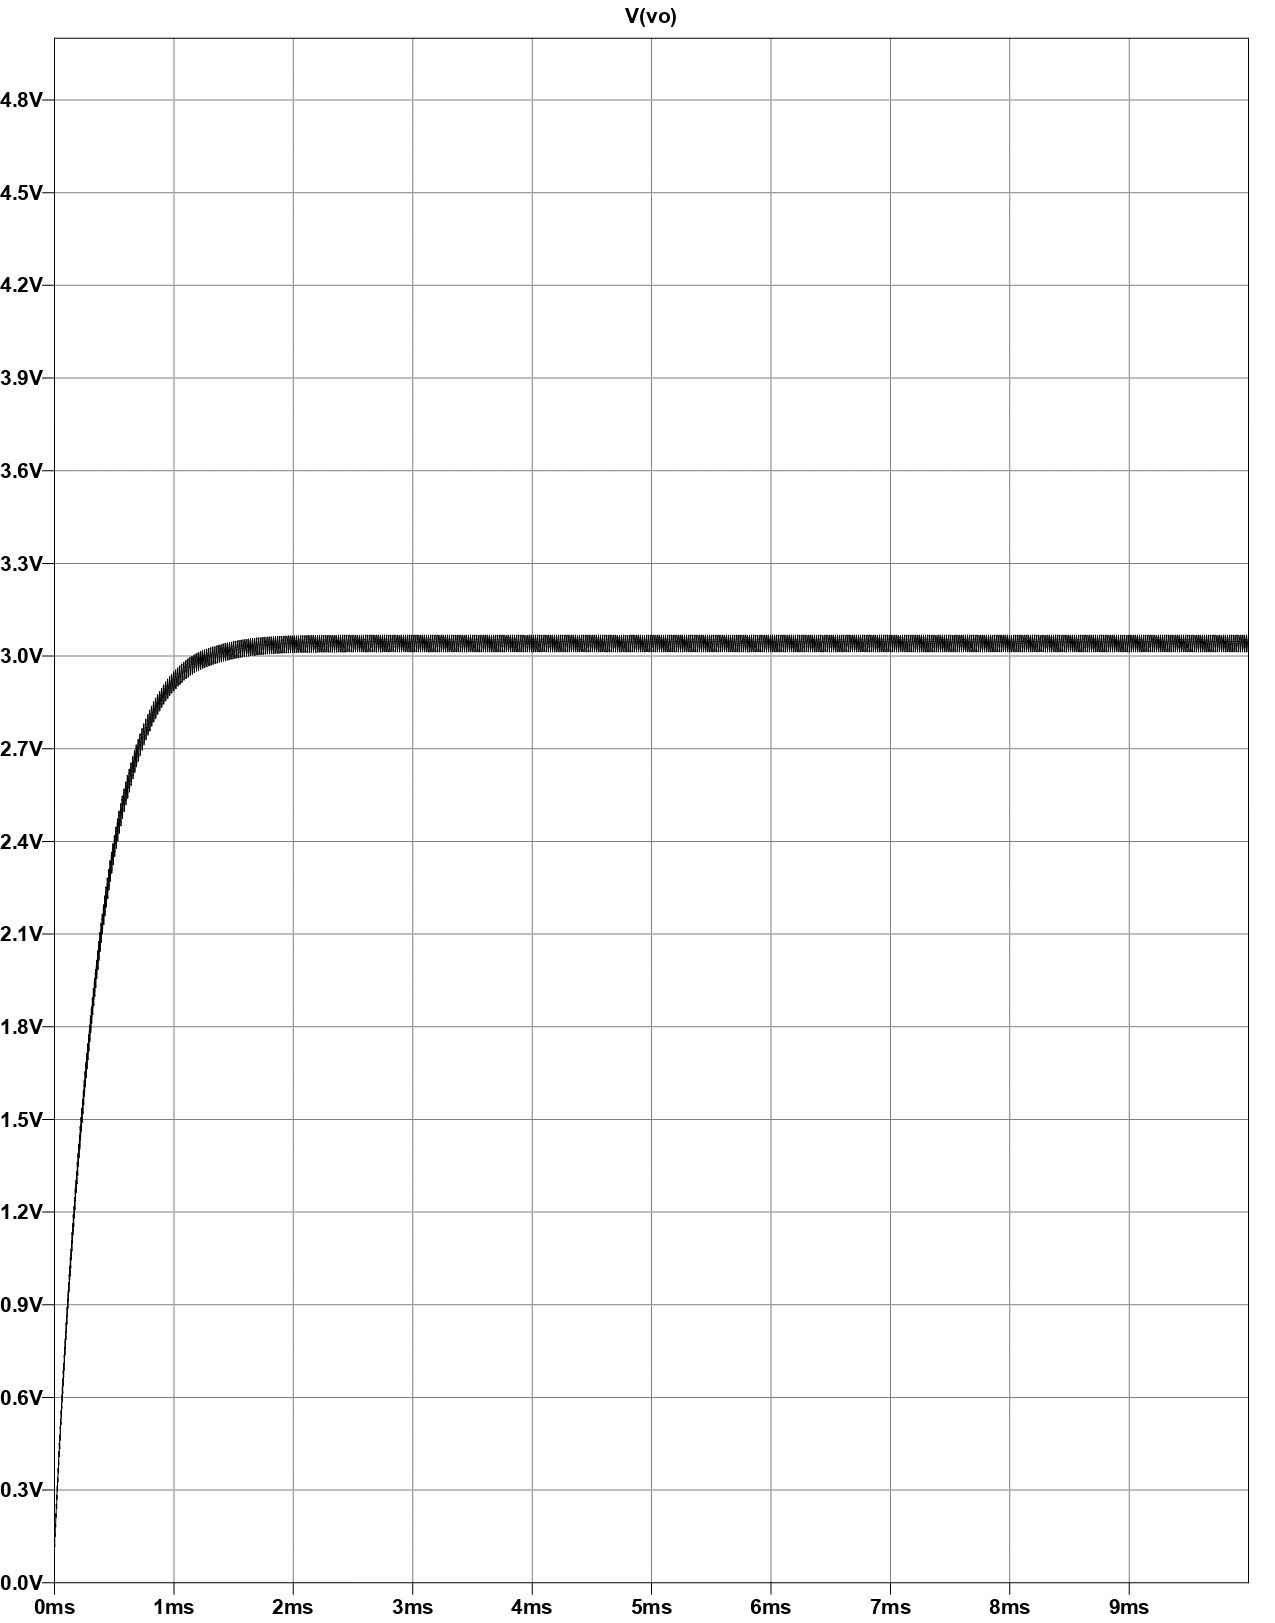
\includegraphics[width=\textwidth]{Pictures/Convertidor DC-DC MC34063A, 2s2p, bus 5.0 v a 500 mA_page-0001 Min.jpg}
    \caption{Salida de voltaje a 5.0 voltios. Vin mínimo operativo (5.5 V).}
    \label{fig:2s2p_50v_2dcdcconverters_min}
  \end{subfigure}
  \caption{Convertidor DC-DC MC34063A, arreglo 2s2p, bus de 5.0 V a 500 mA.}
  \label{fig:arreglo2s2p5vdc}
\end{figure}







% ARREGLO 1S4P
\subsection{Arreglo de baterías 1s4p}

Para esta configuración, es crucial considerar detenidamente la curva de descarga característica de una batería de litio. El fabricante, en el caso del modelo Panasonic NCR-18650B, proporciona una curva tentativa \cite{panasonic_18650b}. Sin embargo, para obtener mediciones más realistas, se requiere realizar pruebas de laboratorio. En este caso, nos apoyamos en las curvas de descarga a una temperatura ambiente de 20°C, obtenidas y evidenciadas en trabajos como el de Kopczynski en 2018 \cite{Kopczynski2018}. Estas mediciones se presentan en la Fig. \ref{fig:discharging_characteristic}.

\begin{figure}[h]
  \centering
  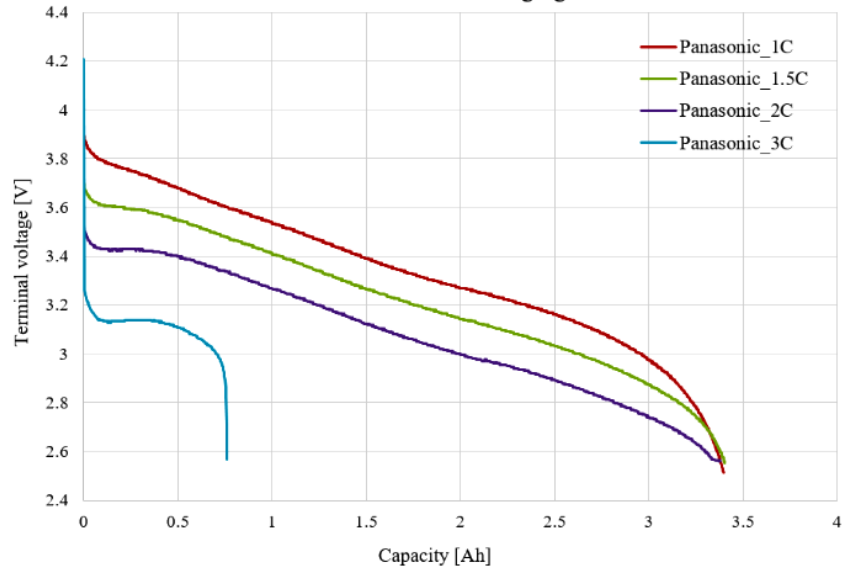
\includegraphics[width=0.45\linewidth]{Pictures/PanasonicCurveDischarge.png} 
  \caption{Discharging characteristic of Panasonic NCR-18650B battery with different discharging current at room temperature (20°C). Fuente: Adaptado de \cite{Kopczynski2018}, con licencia CC BY 4.0}
\label{fig:discharging_characteristic}
\end{figure}

\newpage

Como se evidencia en la Fig. \ref{fig:discharging_characteristic}, una configuración exclusivamente de reducción (buck) o exclusivamente de elevación (boost) resultaría insuficiente. Es en este punto donde surge la necesidad de implementar un convertidor DC-DC que pueda operar dinámicamente en ambos modos. Sin embargo, este enfoque implicaría un nivel de complejidad que excede el alcance de este trabajo de investigación. 

La implementación de tal sistema requeriría la utilización de un circuito integrado distinto al MC34063A, así como un diseño sustancialmente diferente. Por lo tanto, dadas las actuales exigencias del sistema de energía para una misión de globo de gran altitud (HAB), se ha decidido no explorar esta configuración del banco de baterías en el presente estudio.

\vspace{0.75 cm}

\subsection{Implementación de MC34063A en PCB}
\vspace{0.25 cm}
Luego de una minuciosa evaluación del convertidor DC-DC MC34063A en las configuraciones 4s1p, 2s2p y 1s4p, basada en los resultados detallados de las simulaciones en LTSPICE, se llega a la conclusión de que la configuración 4s1p presenta la respuesta más destacada. Tras ajustes precisos en la inductancia del filtro pasabajos, esta disposición exhibió un rendimiento excepcional en la salida, alcanzando el valor de voltaje requerido con un margen de error y un sobreimpulso prácticamente despreciables. Por consiguiente, se ha optado por seleccionar esta configuración para la implementación.

La ejecución de la implementación se llevará a cabo mediante el uso del software Fusion360 de Autodesk. Este programa se utilizará para el desarrollo del esquemático, el diseño de la PCB y el modelado 3D del convertidor DC-DC destinado al bus de 3.3V y 5.0V.\\\\ En las Figuras \ref{fig:MC34063A_Esquemático_33V}, \ref{fig:MC34063A_PCB_33V}, y \ref{fig:MMC34063A_3D_33V}, se presentan detalladamente los resultados obtenidos para el bus de 3.3V.


\newpage

\begin{figure}[h]
  \centering
  \includegraphics[width=0.9\linewidth]{Pictures/MC34063A_Esquemático_33V.png} 
  \caption{Esquemático del convertidor DC-DC con MC34063A. Entrada nominal de 14.4V, salida de 3.3V a 750 mA.}
  \label{fig:MC34063A_Esquemático_33V}
\end{figure}

\begin{figure}[h]
  \centering
  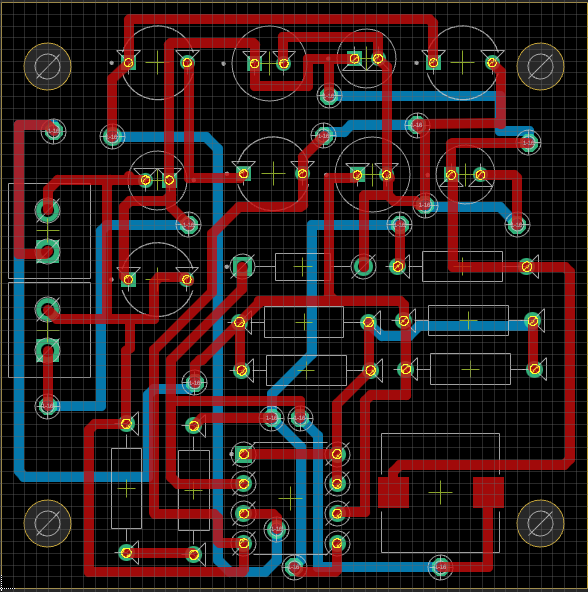
\includegraphics[width=0.52\linewidth]{Pictures/MC34063A_PCB_33V.png} 
  \caption{Diseño de PCB para el convertidor DC-DC con MC34063A. Entrada nominal de 14.4V, salida de 3.3V a 750 mA.}
  \label{fig:MC34063A_PCB_33V}
\end{figure}

\newpage

\begin{figure}[h]
  \centering
  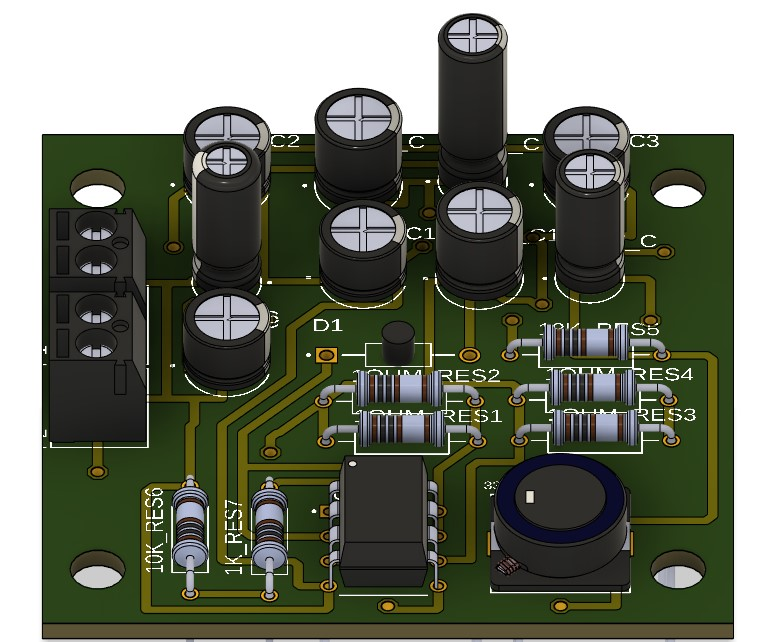
\includegraphics[width=0.65\linewidth]{Pictures/MC34063A_3D_33V.jpeg} 
  \caption{Vista 3D de la PCB para el convertidor DC-DC con MC34063A. Entrada nominal de 14.4V, salida de 3.3V a 750 mA.}
  \label{fig:MMC34063A_3D_33V}
\end{figure}

Para el bus de 5.0V, se desarrollaron el esquemático, la PCB y modelado 3D del convertidor DC-DC, y se presentan en las Figuras \ref{fig:MC34063A_Esquemático_50V}, \ref{fig:MC34063A_PCB_50V} y \ref{fig:MC34063A_3D_50V}, respectivamente.






\begin{figure}[h]
  \centering
  \includegraphics[width=0.9\linewidth]{Pictures/MC34063A_Esquemático_50V.png} 
  \caption{Esquemático del convertidor DC-DC con MC34063A. Entrada nominal de 14.4V, salida de 5.0V a 750 mA.}
  \label{fig:MC34063A_Esquemático_50V}
\end{figure}

\newpage

\begin{figure}[h]
  \centering
  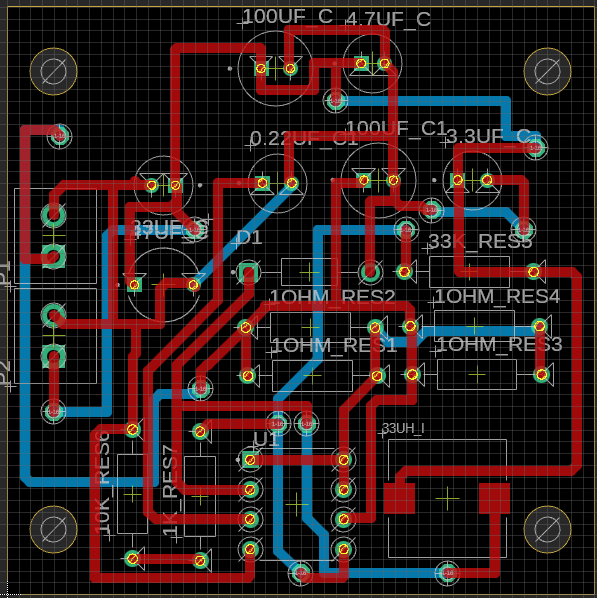
\includegraphics[width=0.55\linewidth]{Pictures/MC34063A_PCB_50V.png} 
  \caption{Diseño de PCB del convertidor DC-DC con MC34063A. Entrada nominal de 14.4V, salida de 5.0V a 750 mA.}
  \label{fig:MC34063A_PCB_50V}
\end{figure}

\begin{figure}[h]
  \centering
  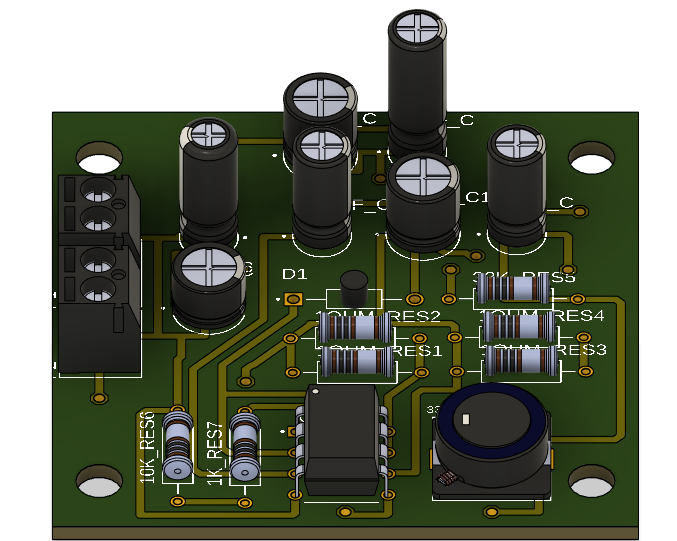
\includegraphics[width=0.75\linewidth]{Pictures/MC34063A_3D_50V.png} 
  \caption{Vista 3D del diseño del convertidor DC-DC con MC34063A. Entrada nominal de 14.4V, salida de 5.0V a 750 mA.}
  \label{fig:MC34063A_3D_50V}
\end{figure}

\newpage

\section{Revisión de autoconsumo de EPS}

Tras dimensionar los componentes del EPS, es crucial evaluar el autoconsumo por dos razones: validar el dimensionamiento inicial del banco de baterías y determinar la corriente efectiva de los convertidores DC-DC. Los detalles del consumo energético se encuentran en las Tablas \ref{tab:autoconsumo50_EPS} y \ref{tab:autoconsumo33_EPS}.




\begin{table}[!ht]
    \centering
    \renewcommand{\arraystretch}{1.2}
    \caption{Cuadro de cargas para autoconsumo de EPS, bus 5.0 V}
    \label{tab:autoconsumo50_EPS}
    \begin{tabularx}{1.1\textwidth}{lllllll}
    \hline
    \textbf{Descripción} & \textbf{Cantidad} & \textbf{I [mA]} & \textbf{P [W]} & \textbf{t [h]} & \textbf{E [Wh]} & \textbf{Q [mAh]} \\
    \hline
    MCU & 1 unidad & 180.00 & 0.900 & 6.00 & 5.40 & 1080.00 \\ 
    MOSFET & 1 unidad & 33.00 & 0.165 & 6.00 & 0.99 & 198.00  \\ 
    MS5611 & 1 unidad & 1.4 & 0.00 & 6.00 & 0.04 & 8.40  \\ 
    ACS723 & 1 unidad & 1.00 & 0.00& 6.00 & 0.03& 6.00  \\ 
    ADC & 2 unidad & 80.00 & 0.40 & 6.00 & 0.24 & 480.00 \\
    \hline
    & & \textbf{I Máx.} & 295.40 & &\textbf{Q Total.} & 1772.40 \\ 
    \hline
    \end{tabularx}
\end{table}


\begin{table}[!ht]
    \centering
    \renewcommand{\arraystretch}{1.2}
    \caption{Cuadro de cargas para autoconsumo de EPS, bus 3.3 V}
    \label{tab:autoconsumo33_EPS}
    \begin{tabularx}{1.1\textwidth}{lllllll}
    \hline
    \textbf{Descripción} & \textbf{Cantidad} & \textbf{I [mA]} & \textbf{P [W]} & \textbf{t [h]} & \textbf{E [Wh]} & \textbf{Q [mAh]} \\
    \hline
    MOSFET & 1 unidad & 33.00 & 0.01 & 6.00 & 0.6 & 120.00 \\
    \hline
    & & \textbf{I Máx.} & 33.00 & &\textbf{Q Total.} & 120.00 \\ 
    \hline
    \end{tabularx}
\end{table}

En el capítulo III, sección en la que se desarrolló un presupuesto energético, estimamos inicialmente una corriente de 983 mA y un consumo en carga de 5519 mAh para el bus de 3.3 V. Para el bus de 5.0 V, se estimó una corriente de 402 mA y un consumo en carga de 1326 mAh.

Considerando el autoconsumo del EPS (ver la Tabla \ref{tab:autoconsumo50_EPS} y Tabla \ref{tab:autoconsumo33_EPS}), actualizamos estos valores de la siguiente manera: el bus de 3.3 V tendría una corriente de 1016 mA con una necesidad en carga de 5639 mAh. En cuanto al bus de 5.0 V, la corriente sería de 698 mA y la carga de 3098 mAh.

Estas cifras son mejores para dimensionar las protecciones eléctricas. La necesidad total de carga es de 8737 mAh, pero aún no hemos considerado la eficiencia de los convertidores DC-DC (aproximadamente 83.7\% según el fabricante \cite{ti_mc34063a}). Esto nos lleva a una carga necesaria de 10439 mAh. Comparando con la capacidad nominal del arreglo 4s1p de 13600 mAh, concluimos que el banco de baterías sigue siendo capaz, al 77\% de su capacidad.



\section{Dispositivos de Protección Eléctrica}

Las baterías de iones de litio, debido a su alta densidad energética, requieren un manejo cauteloso. En el mercado actual, los circuitos integrados (IC) especializados abordan consideraciones críticas de seguridad, destacando:

\begin{itemize}
    \item \textbf{Sobrecarga:} Las baterías deben cargarse hasta 4.1 V o 4.2 V/celda de manera segura. Un circuito de protección evita daños y riesgos de incendio.
    \item \textbf{Sobre-descarga:} Evita descargar las baterías por debajo de 2.5 V/celda para preservar su vida útil.
    \item \textbf{Descarga rápida:} Los IC desconectan la batería ante corrientes de descarga excesivas.
\end{itemize}

Los IC de protección utilizan MOSFET para gestionar la conexión y desconexión de celdas de litio. Permiten la conexión en paralelo de celdas del mismo tipo, compartiendo eficientemente el circuito de protección \cite{knight2015lithium}.

Para este trabajo de investigación, consideraremos dos alternativas, una orientada al caso de implementar un cargador a bordo, y la otra considerando únicamente el proceso de descarga, es decir un limitador de corriente. Además, como medida de protección adicional, los interruptores mecánicos pueden ser una buena adición al diseño, reduciendo aún más el riesgo de encendidos accidentales del sistema previo a la misión. 

\subsection{Protección eléctrica para cargador a bordo}

Las consideraciones críticas de sobrecarga, sobre-descarga y descarga rápida son abordadas integralmente en este enfoque de protección eléctrica, especialmente diseñado para un flujo bidireccional de potencia, tanto desde el banco de baterías hacia las cargas como del cargador hacia las baterías.

Para la implementación práctica en proyectos de potencia a escala, con énfasis en la economía y accesibilidad, se destaca el uso del circuito integrado AP9101C de Diodes Incorporated.

El AP9101C, un IC de protección altamente preciso, está diseñado para salvaguardar baterías al detectar sobrecargas, sobredescargas y otros eventos anómalos. Su bajo consumo de corriente, precisión en la detección de voltajes y circuito de tiempo incorporado minimizan la necesidad de componentes externos. Se presenta como una opción eficiente y precisa para la protección de baterías. La Tabla \ref{tab:ap9101} detalla sus características. En cuanto al esquemático, el fabricante ofrece una configuración \cite{diodes2023ap9101c}.




\begin{table}[h]
    \centering
    \caption{Parámetros Clave AP9101C}
    \begin{tabular}{l|l}
        \hline
        \textbf{Baja Corriente de Consumo} & \begin{tabular}[c]{@{}l@{}}3.0µA Typ. (Modo de Operación, VDD = 3.5V)\\ 0.01µA Typ. (Modo de Apagado)\end{tabular} \\ \hline
        \textbf{Circuito de Detección de Voltaje} & \begin{tabular}[c]{@{}l@{}}Alta Precisión a +25°C\\ Sobrecarga: 3.5V a 4.5V (±25mV)\\ Sobre descarga: 2.0V a 3.4V (±35mV)\end{tabular} \\ \hline
        \textbf{Rango de Voltaje de Histéresis} & \begin{tabular}[c]{@{}l@{}}Sobrecarga: 0.1V a 0.4V (±50mV)\\ Sobre descarga: 0V a 0.7V (±65mV)\end{tabular} \\ \hline
        \textbf{Sobrecorriente de Descarga} & \begin{tabular}[c]{@{}l@{}}Voltaje de Detección: 0.05V a 0.32V (±15mV)\\ Corriente Corta: 0.45V a 0.7V (±100mV)\end{tabular} \\ \hline
        \textbf{Sobrecorriente de Carga} & \begin{tabular}[c]{@{}l@{}}Voltaje de Detección: -0.2V a -0.05V (±15mV)\\ Detección de Sobrecargador: 8.0V (Fijo, ±2V)\\ Liberación de Sobrecargador: 7.3V (Fijo, ±2V)\end{tabular} \\ \hline
    \end{tabular}
    \label{tab:ap9101}
\end{table}

\begin{figure}[h]
  \centering
  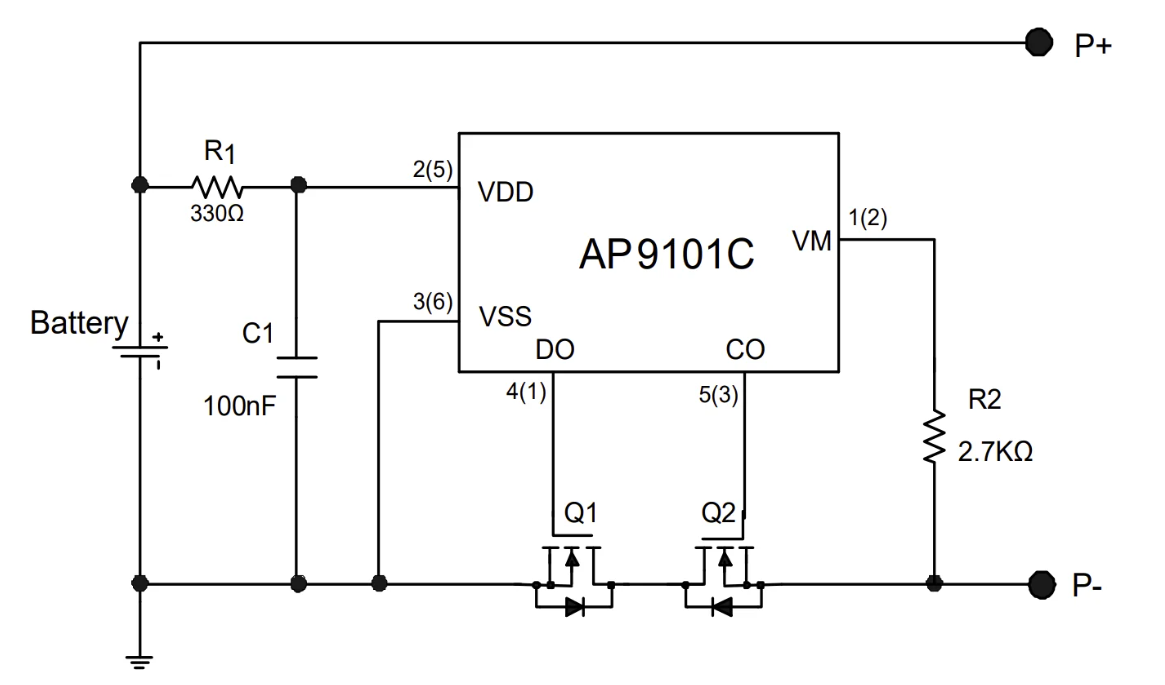
\includegraphics[width=\linewidth]{Pictures/AP9101C.png} 
  \caption{Esquemático de circuito de protección AP9101C \cite{diodes2023ap9101c}. Los valores son los sugeridos por el fabricante. El modelo MOSFET se recomienda el modelo DMG6968 de Diodes Incorporated.}
  \label{fig:EsquematicoAP9101C}
\end{figure}

\newpage
\subsection{Protección eléctrica como limitador de corriente}

En el contexto de una misión de globo de gran altitud con un período operativo breve, donde no se realizarán ciclos de carga y descarga del banco de baterías, se buscan protecciones específicas. Dado que el escenario se limita principalmente a la descarga de las baterías, las medidas de protección se orientan hacia la preparación ante eventos como cortocircuitos. Una alternativa adecuada es la implementación de circuitos conocidos como limitadores de corriente, como el IC comercial LTC4361 de Analog Devices \cite{LTC4361}, el cual utilizaremos en este trabajo. Las especificaciones técnicas de este dispositivo se detallan en la Tabla \ref{tab:especificaciones_LTC4361}.




\begin{table}[h]
  \centering
  \caption{Especificaciones de LTC4361}
  \begin{tabular}{l|l}
    \hline
    \textbf{Característica} & \textbf{Valor} \\
    \hline
    Rango de Operación & 2.5V a 5.5V \\
    Protección contra Sobretensión & Hasta 80V \\
    No se Requiere Condensador de Entrada o TVS & Para la mayoría de las aplicaciones \\
    Umbral de Sobretensión Preciso & 5.8V con 2\% de precisión \\
    Interruptor de Circuito de Sobrecorriente & 50mV con 10\% de precisión \\
    Apagado por Sobretensión <1µs & Apagado suave \\
    \hline
  \end{tabular}
  \label{tab:especificaciones_LTC4361}
\end{table}

Para la implementación del LTC4361, la hoja técnica propone un esquemático y establece que el dispositivo regula su valor de disparo para la protección mediante un ajuste de corriente, que se determina a partir de la ecuación \ref{eq:LTC4361}.

\begin{equation}\label{eq:LTC4361}
    R_{\text{sense}} = \frac{\Delta V_{\text{oc}}}{I_{\text{trip}}}
\end{equation}


Donde:
\begin{itemize}
    \item $\Delta V_{\text{oc}}$ tiene un valor de 50mV.
    \item $I_{\text{trip}}$ es la corriente de disparo.
\end{itemize}

Sabemos que la corriente de operación estimada para el bus de 3.3 V es de 1016 mA, mientras que para el bus de 5.0 V es de 698 mA. Sin embargo, la consideración de esta información no es el único aspecto crucial. También debemos tener en cuenta que el diseño de las protecciones se orienta a prevenir daños en los sistemas electrónicos. En particular, se enfoca en proteger el material conductor, que en este caso corresponde a las pistas de los circuitos. Para este trabajo, se ha tomado un espesor general de 0.762 mm o 30 milésimas de pulgada (mil) para cada diseño de PCB.

Este valor se seleccionó considerando el material utilizado, que es FR-4. Según la tabla proporcionada por la compañía Altium para PCB con material FR-4, que sigue la norma definida por la NEMA (National Electrical Manufacturers Association) para un compuesto de resina epoxídica reforzada con fibra de vidrio, el espesor de 0.762 mm corresponde a una capacidad de corriente de 2 A. Esta información detallada se puede consultar en la Tabla \ref{tab:relacion_corriente_grosor}, que ofrece una referencia específica para el diseño de las pistas.

\begin{table}[h]
    \centering
    \caption{Relación entre la corriente y el grosor de la pista.}
    \label{tab:relacion_corriente_grosor}
    \begin{tabular}{ll}
        \hline
        Corriente (A) & Grosor de pista (mil) \\ 
        \hline
        1 & 10 \\ 
        2 & 30 \\ 
        3 & 50 \\ 
        4 & 80 \\ 
        5 & 110 \\ 
        6 & 150 \\ 
        7 & 180 \\ 
        8 & 220 \\ 
        9 & 260 \\ 
        10 & 300 \\ 
        \hline
    \end{tabular}
\end{table}

Dicho esto, se tomará un punto intermedio entre la capacidad de las pistas en las PCB (2 amperios) y la corriente estimada en el bus de mayor demanda (1 amperio). Por lo tanto, la corriente configurada como sobrecorriente o corriente de disparo de protecciones será de 1.5 amperios. Dando como resultado de la \ref{eq:LTC4361} un valor de $R_{sense}$ de 0.33 ohm.

Una vez definida la corriente de disparo, el esquemático está completo de acuerdo con la hoja técnica del fabricante \cite{LTC4361}, ver Fig. \ref{fig:Esquematico_LTC4361}, el diseño 2D de la PCB en la Fig. \ref{fig:PCB_LTC4361}y la vista 3D en la Fig.\ref{fig:3D_LTC4361}. 

\newpage

\begin{figure}[h]
  \centering
  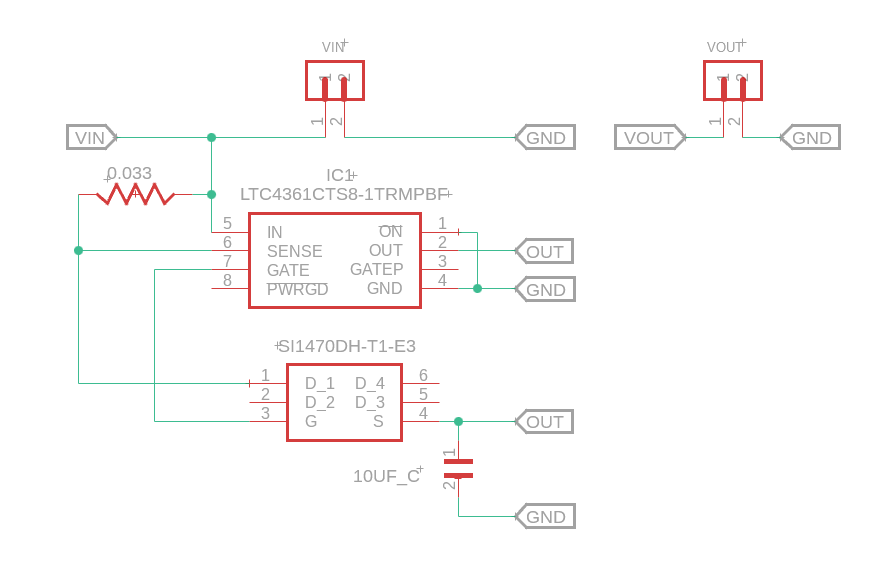
\includegraphics[width=\linewidth]{Pictures/Esquematico_LTC4361.png} 
  \caption{Esquemático de circuito de protección LT4361 \cite{LTC4361}. Los valores son los sugeridos por el fabricante. Se calculó \(R_{\text{sense}} = 0.33 \ \Omega\) para \(I_{\text{trip}} = 1.5 \ \text{A}\).}
  \label{fig:Esquematico_LTC4361}
\end{figure}
\vspace{1 cm}
\begin{figure}[h]
  \centering
  \begin{subfigure}[b]{0.55\textwidth}
    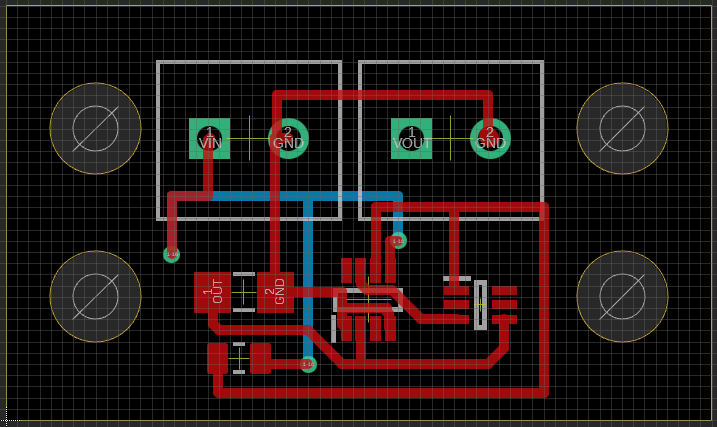
\includegraphics[width=\linewidth]{Pictures/PCB_LTC4361.png}
    \caption{PCB de circuito de protección LTC4361}
    \label{fig:PCB_LTC4361}
  \end{subfigure}%
  \begin{subfigure}[b]{0.55\textwidth}
    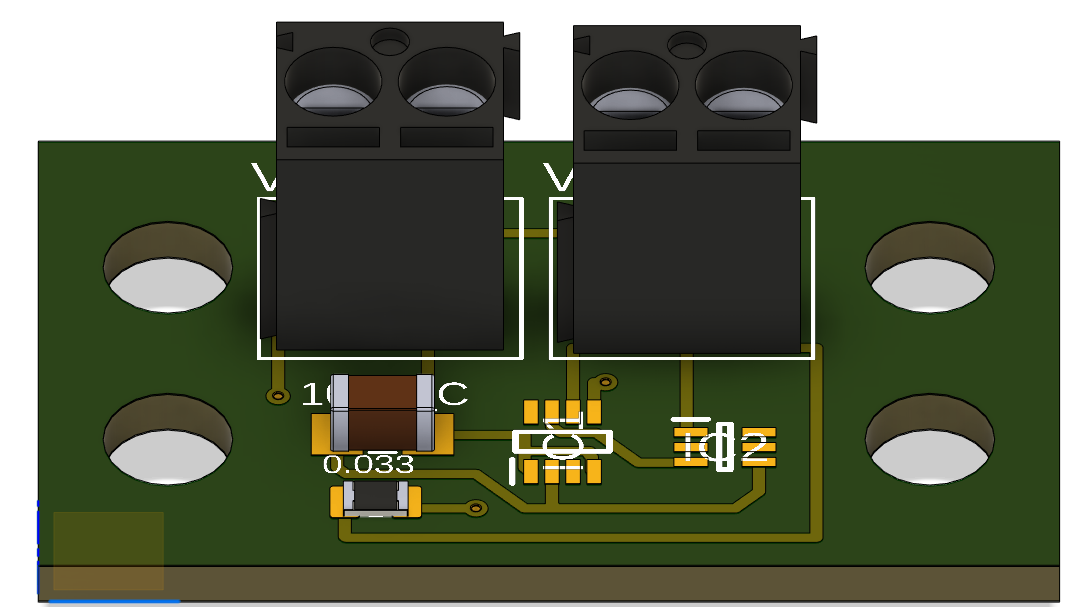
\includegraphics[width=\linewidth]{Pictures/3D_LTC4361.png}
    \caption{Vista 3D de PCB de protección LTC4361}
    \label{fig:3D_LTC4361}
  \end{subfigure}
  \caption{PCB y Vista 3D del circuito de protección LTC4361}
  \label{fig:combinada_LTC4361}
\end{figure}

\newpage
\subsection{Sistemas de Desconexión y Seguridad}

En esta categoría, se exploran dos mecanismos esenciales. El primero consiste en un interruptor de 4 polos con 2 posiciones para cada uno (Fig. \ref{fig:4polosinterruptor}). Este diseño permite la desconexión individual de cada pila 18650, brindando la capacidad de aislar completamente el banco de baterías del resto del circuito y entre el arreglo de las pilas mismas.

\begin{figure}[h]
  \centering
  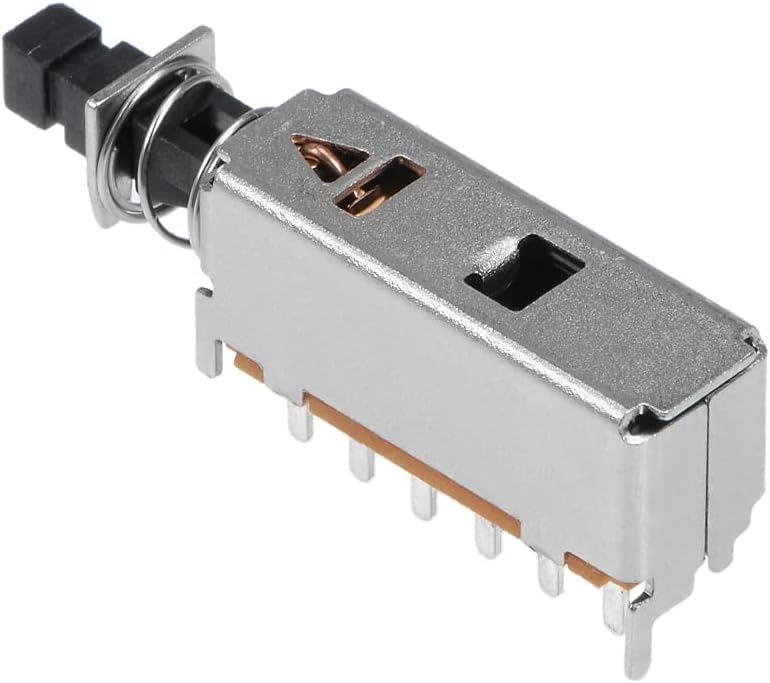
\includegraphics[width=0.3\linewidth]{Pictures/Interruptor.jpg} 
  \caption{Interruptor de 4 polos uxcell}
  \label{fig:4polosinterruptor}
\end{figure}

Como segundo sistema de seguridad, se implementa un enfoque similar al utilizado en misiones espaciales: un interruptor 'Remove Before Flight' (Fig. \ref{fig:figuraPrincipal}). Este interruptor actúa como un punto de control adicional contra posibles fallos y para prevenir activaciones no deseadas del sistema. Su adopción se basa en las mejores prácticas de seguridad y la experiencia acumulada en entornos críticos, donde prevenir errores humanos es de suma importancia.

\begin{figure}[h]
  \centering
  \begin{subfigure}{0.3\linewidth}
    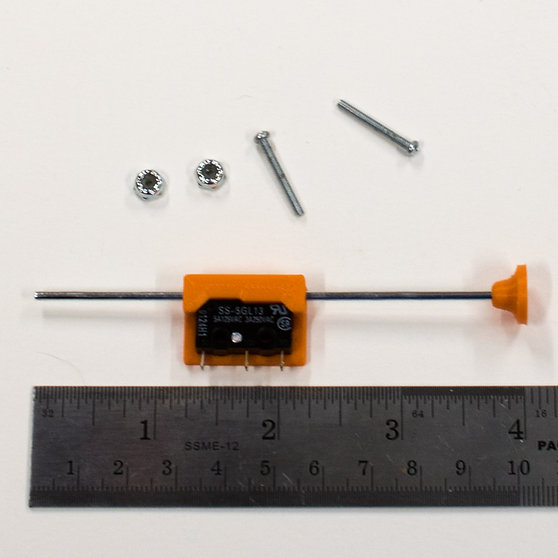
\includegraphics[width=\linewidth]{Pictures/rbfinterruptor.jpg}
    \caption{Configuración}
    \label{fig:subfiguraA}
  \end{subfigure}
  \hspace{1cm} % Espacio horizontal entre las subfiguras
  \begin{subfigure}{0.3\linewidth}
    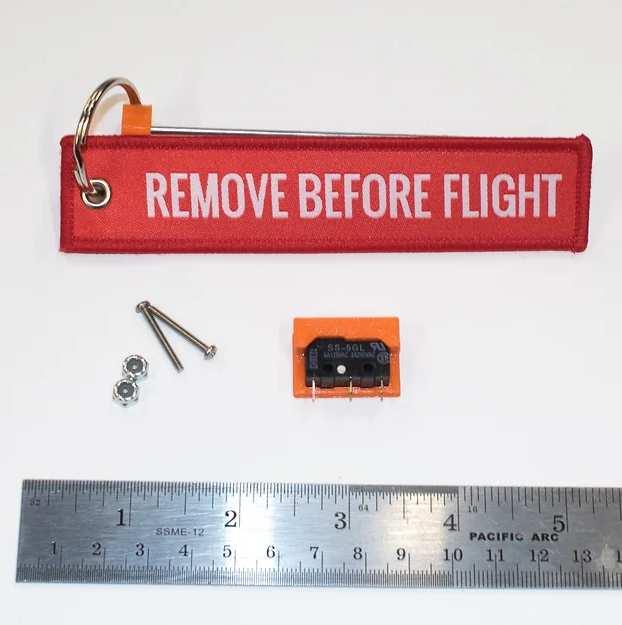
\includegraphics[width=\linewidth]{Pictures/rbfitems.png}
    \caption{Elementos}
    \label{fig:subfiguraB}
  \end{subfigure}
  \caption{Interruptor "Remove before flight \cite{labralab_pull_pin_switch_kit_2023}}
  \label{fig:figuraPrincipal}
\end{figure}

Ambos mecanismos de protección se conectan en serie, lo que implica que deben activarse secuencialmente para permitir el funcionamiento del sistema. Esta configuración en serie garantiza un doble nivel de seguridad, ya que ambas barreras deben superarse manualmente antes de que el sistema pueda operar.








